%! Author = ibw
%! Date = 09.11.23

% Preamble
\section{Evaluation}
\subsection{Exkurs Architektur}
%! Author = itgramic
%! Date = 05.12.23

% Preamble
\subsubsection{Monolithische vs. verteilte SQL Systeme}
Klassische SQL-Datenbanken sind Monolithische Systeme, selbst wenn sie mittels Replikation eine Primary/Standby-Architektur aufweisen.
Man kann mittels eines SQL Proxys ein gewisses Mass an Load Balancing betreiben, hat aber immer noch das Problem das es einen Primary Node gibt auf dem beschrieben wird.

Verteilte Systeme wiederum

\begin{figure}[H]
    \centering
    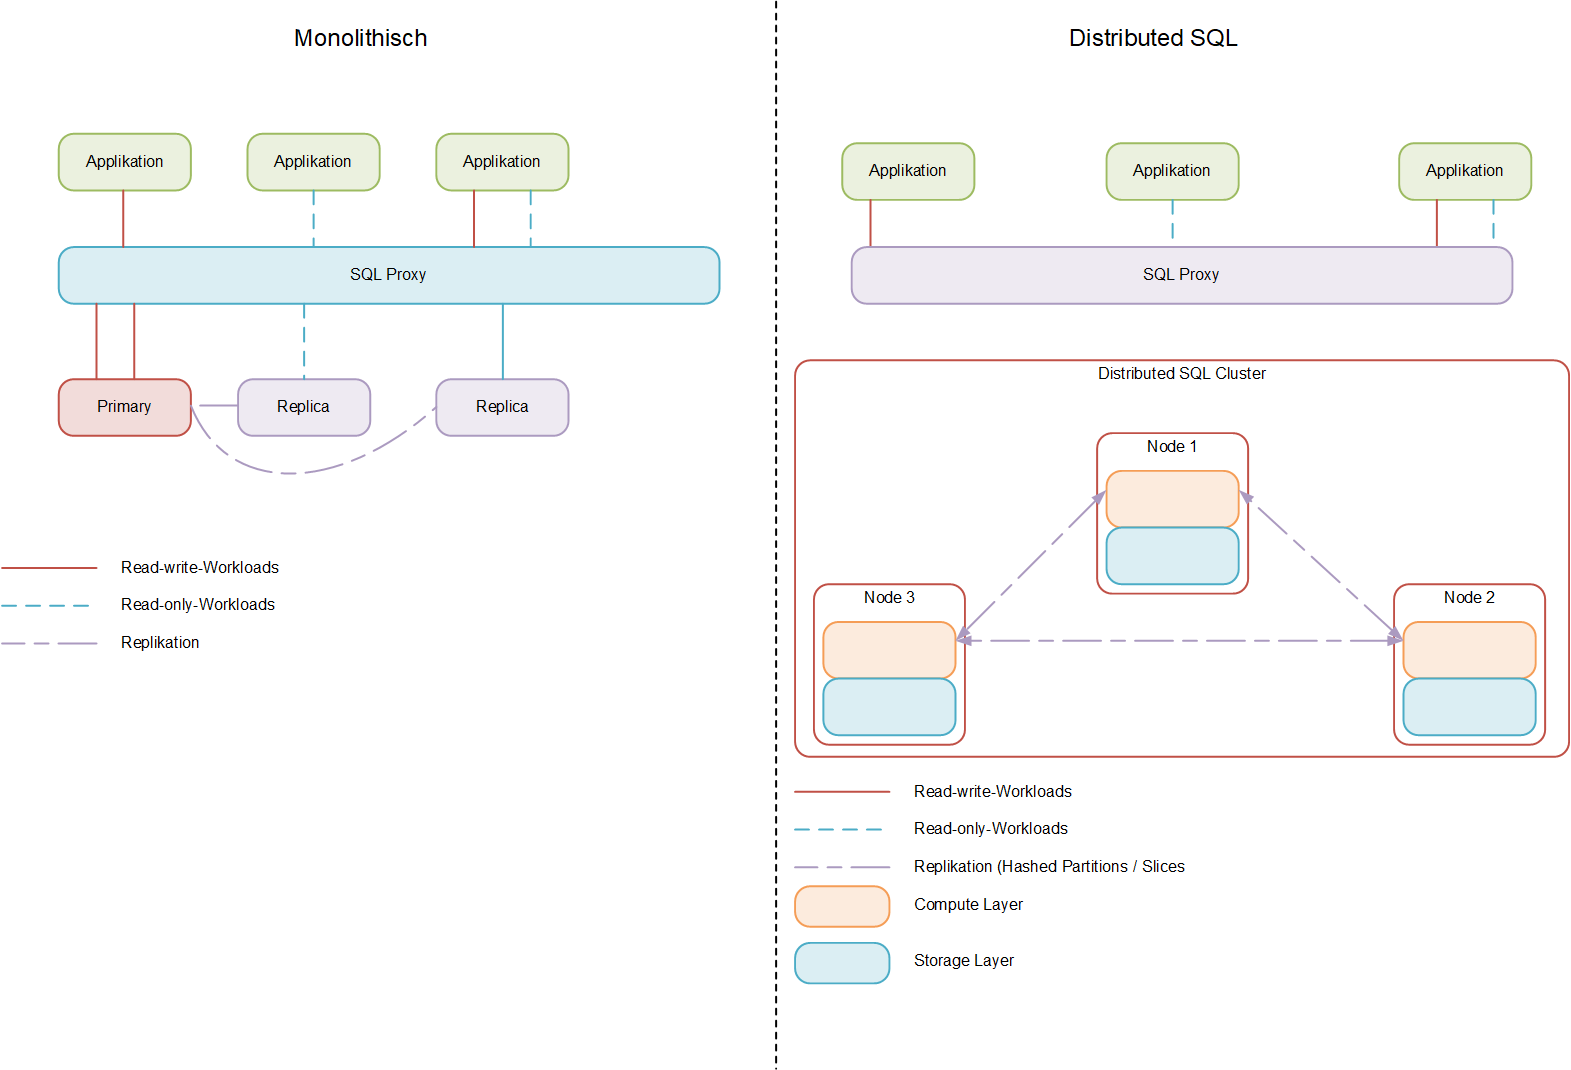
\includegraphics[width=1\linewidth]{source/implementation/evaluation/excursus_architecture/monolith_distributed}
    \caption{Monolithische vs. verteilte SQL Systeme}
    \label{fig:Monolith_vs_Distributed_SQL}
\end{figure}

%! Author = itgramic
%! Date = 05.12.23

% Preamble
\subsubsection{High Availability und Replikation}
\begin{flushleft}
    Wenn eine Datenbank HA (High Availability), also Hochverfügbar, sein soll, braucht es eine Primäre und mindestens eine Sekundäre- oder \Gls{Failover}-Datenbank.
    Um Datenverlust zu vermeiden, müssen die Daten permanent von der Primären auf die sekundäre Datenbank repliziert werden, dies nennt man Replikation\cite{D9RDXENY}.
    Dabei wird zwischen den folgenden beiden Replikationen unterschieden:
\end{flushleft}
\begin{flushleft}
    \textbf{Synchrone Replikation}\\
    Wenn bei einer Synchronen Replikation eine Transaktion abgesetzt wird, wird der Commit auf der primären Seite erst gesetzt, wenn die Änderung auf der sekundären Seite oder den sekundären Seiten ebenfalls eingetragen und Committed ist.
    Bis zu diesem Moment ist die Transaktion nicht als Committed.
    
    Dies wird dann zum Problem, wenn keine Verbindung mehr zu mindesten einer sekundären Seite vorhanden ist.
    Zudem wird die Synchrone Replikation bei hohen Latenzen zum Bottleneck der Datenbank.
\end{flushleft}
\begin{flushleft}
    \textbf{Asynchrone Replikation}\\
    Bei der Asynchronen Replikation wird eine Transaktion erst auf der eigenen primären Seite Committed und erst dann an die sekundären Nodes gesendet.
    Besonders bei hohen Latenzen bleibt die Datenbank immer perfomant, allerdings kann es je nach Latenz und genereller Auslastung zu Datenverlusten kommen, wenn es zum \Gls{Failover} kommt.
\end{flushleft}
%! Author = itgramic
%! Date = 05.12.23

% Preamble
\subsubsection{Quorum}
\label{subsubsec:quorum}
\begin{flushleft}
    Ein Quorum-System soll die Integrität und Konsistenz in einem Datenbank-Cluster sicherstellen.
    Dabei gilt zu beachten, das nicht eine beliebige Anzahl an Nodes hinzugefügt werden können.
    Auch hat das Hinzufügen von Nodes immer eine Einbusse an Performance zur Folge, besonders dann, wenn eine synchrone Replikation gewählt wird und auf jedes Commitment von den Replica-Nodes gewartet werden muss.

    \begin{description}
        \item \textbf{Quorum}\hfill \\Die Mehrheit der Server, die einen funktionierenden Betrieb gewährleisten können, ohne eine \Gls{Split-brain}-Situation zu erzeugen.
        Die Formel ist gemeinhin \(n/2 + 1\)
        \item \textbf{Throughput}\hfill \\Beschreibt, wie sich die Anzahl Nodes auf die Schreibgeschwindigkeit der Commitments auf die restlichen Nodes auswirkt.\\Die Verdopplung der Server halbiert i. d. R. den Throughput.
        \item \textbf{Fehlertoleranz}\hfill \\Beschreibt, wie viele Nodes ausfallen können, damit der Cluster noch arbeitsfähig ist.\\Wobei eine Erhöhung der Nodes von 3 auf 4 die Fehlertoleranz nicht erhöht, da nun eine \Gls{Split-brain}-Situation entstehen kann.
    \end{description}
    %\begin{landscape}
    %\begin{table}[]
    %\resizebox{\columnwidth}{!}{%
    %\begin{tabular}{@{}llll@{}}
    %\toprule
    %\textbf{Anzahl Nodes} & \textbf{Quorum} & \textbf{Fehlertoleranz} & \textbf{Representative Throughput} \\ \midrule
    %1                     & 1               & 0                                               & 100                                \\
    %2                     & 2               & 0                                               & 85                                 \\
    %3                     & 2               & 1                                               & 82                                 \\
    %4                     & 3               & 1                                               & 57                                 \\
    %5                     & 3               & 2                                               & 48                                 \\
    %6                     & 4               & 2                                               & 41                                 \\
    %7                     & 4               & 3                                               & 36                                 \\ \bottomrule
    %\end{tabular}%
    %}
    %\caption{Quorum Beispiele}
    %\label{tab:quorum-beispiele}
    %\end{table}
    %\end{landscape}
    %\subsubsection{Split-brain}
    %\label{chap:Split-brain}
    Hier ein Beispiel wie sie in den Artikeln \cite{UMIGLCCI, YDS7DTYM, V4XLXN7W} beschrieben werden.
    Es zeigt auf, ab wie vielen Nodes die Fehlertoleranz erhöht wird und wie sich der repräsentative Throughput verhält.
%\end{flushleft}
%\begin{flushleft}
    \begin{table}[H]
    \resizebox{\columnwidth}{!}{%
    \begin{tabular}{@{}llll@{}}
    \toprule
    \textbf{Anzahl Nodes} & \textbf{Quorum} & \textbf{Fehlertoleranz} & \textbf{Representative Throughput} \\ \midrule
    1                     & 1               & 0                       & 100                                \\
    2                     & 2               & 0                       & 85                                 \\
    3                     & 2               & 1                       & 82                                 \\
    4                     & 3               & 1                       & 57                                 \\
    5                     & 3               & 2                       & 48                                 \\
    6                     & 4               & 2                       & 41                                 \\
    7                     & 4               & 3                       & 36                                 \\ \bottomrule
    \end{tabular}%
    }
    \caption{Quorum Beispiele}
    \label{tab:quorum-beispiele}
    \end{table}
\end{flushleft}
%! Author = itgramic
%! Date = 05.12.23

% Preamble
\subsubsection{CAP Theorem}
Das CAP Theorem besagt, das nur zwei der drei folgenden drei Merkmale von verteilten Systeme gewährleistet werden können\cite{EE6EQHU2}.
\begin{flushleft}
\textbf{Konsistenz - Consistency}\\
    Die Datenbank ist Konsistent, alle Clients seher gleichzeitig die gleichen Daten unabhängig auf welchem Node Zugegriffen wird.
    Hierzu muss eine Replikation der Daten an alle Nodes stattfinden und der Commit zurückgegeben werden, also eine Synchrone Replikation stattfinden.
\end{flushleft}
\begin{flushleft}
\textbf{Verfügbarkeit - Availability}\\
    Jeder Client, der eine Anfrage sendet, muss auch eine Antwort erhalten.
    Unabhängig davon wie viele Nodes im Cluster noch aktiv ist.
\end{flushleft}
\begin{flushleft}
\textbf{Ausfalltoleranz / Partitionstoleranz - Partition tolerance}\\
    Der Cluster muss auch dann noch funktionsfähig bleiben, wenn es eine beliebige Anzahl von Verbindungsunterbrüchen oder anderen Netzwerkproblemen zwischen den Nodes gibt.

\end{flushleft}
\begin{flushleft}
    \begin{figure}[H]
        \centering
        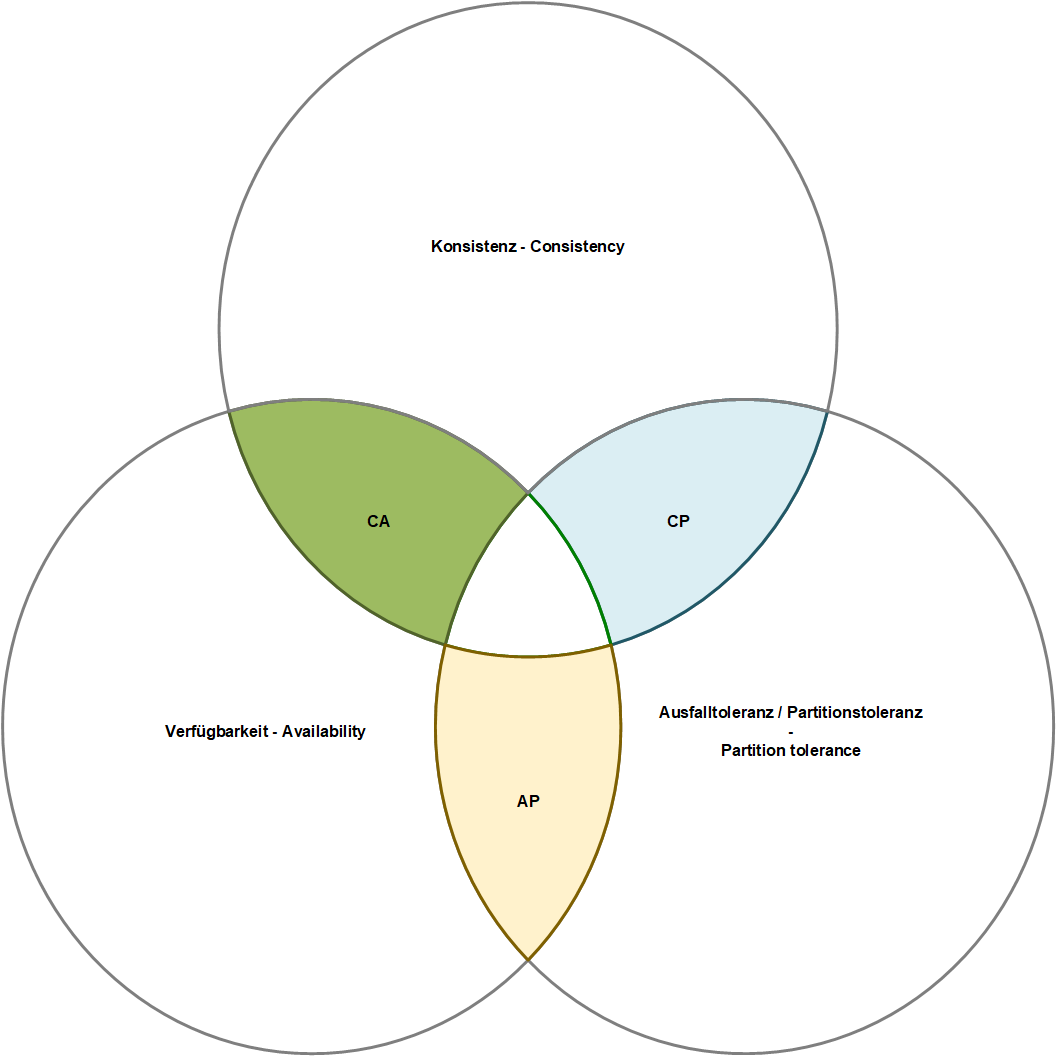
\includegraphics[width=0.5\linewidth]{source/implementation/evaluation/excursus_architecture/cap_theorem}
        \caption{CAP-Theorem}
        \label{fig:cap_theorem}
    \end{figure}

    \Gls{PostgreSQL}, \Gls{Oracle Database} oder \Gls{IBM DB2} präferieren CA, also Konsistenz und Verfügbarkeit.
\end{flushleft}
%! Author = itgramic
%! Date = 05.12.23

% Preamble
\subsubsection{Skalierung}
Datenbanken müssen skalierbar sein.
Dabei wird unterschieden zwischen einer vertikalen Skalierung (scale-up) und horizontaler Skalierung (scale-out).
Bei der vertikalen Skalierung werden den DB-Servern mehr CPU-Cores und Memory sowie zum Teil Storage hinzugefügt, wobei der Storage in jedem Fall wachsen wird.
Beim horizontalen Skalieren werden weitere DB-Nodes in den Cluster eingehängt\cite{IZSGZLVT}:
\begin{figure}[H]
    \centering
    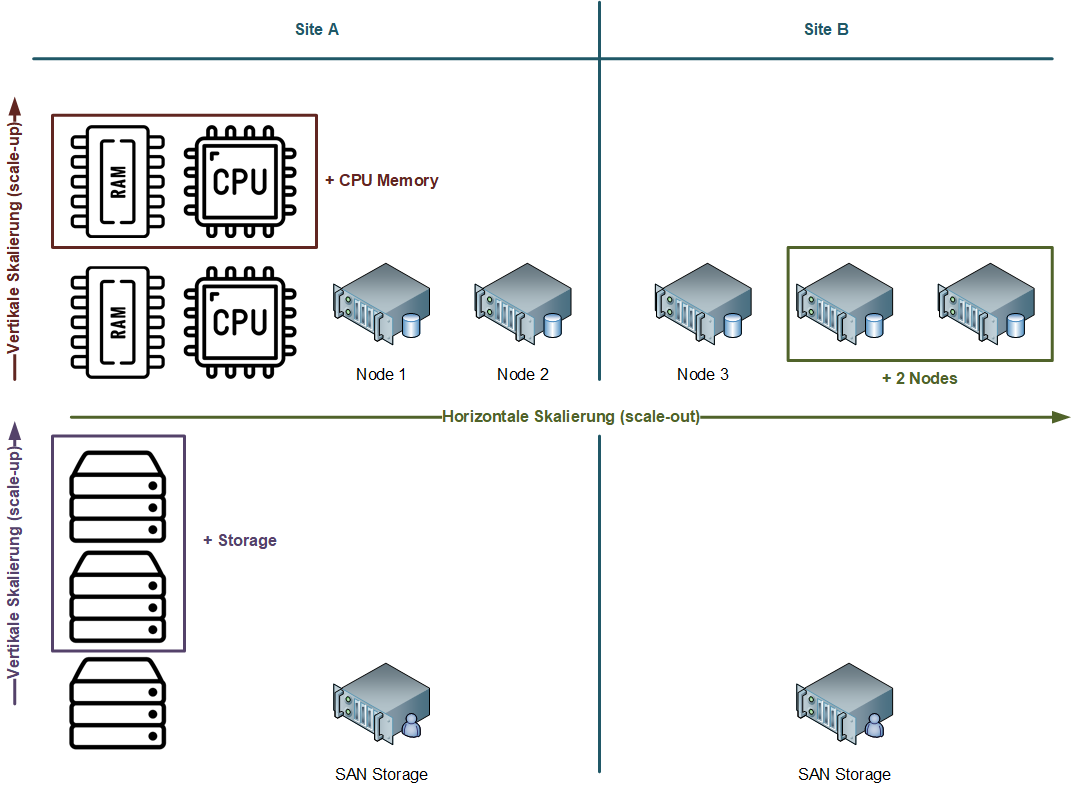
\includegraphics[width=1\linewidth]{source/implementation/evaluation/excursus_architecture/Skalierung}
    \caption{Datenbankskalierung}
    \label{fig:Datenbankskalierung}
\end{figure}

Bei monolithischen Datenbanken, werden irgendwann die grenzen der horizontalen Skalierung erreicht und man muss wieder vertikal Skalieren, um dem Primary Node genügend Rechnerleistung vorzuhalten.
\subsection{Erheben und Gewichten der Anforderungen}
%! Author = itgramic
%! Date = 29.12.23

% Preamble
\subsubsection{Anforderungen}
\begin{flushleft}
    Das KSGR hat eine Cloud First Strategie.\\
    Das heisst, alle neuen Applikationen und entsprechend deren Datenbanken müssen Cloud Ready bzw.
    Cloud Native sein.
    Um die Voraussetzung dafür zu schaffen, muss auch der PostgreSQL Cluster Cloud Ready sein.
\end{flushleft}
\begin{flushleft}
    Daher müssen zwei von drei genauer evaluierten Lösungen Cloud Native Lösungen sein.
    Wenn der Zeitaufwand reicht, können auch eine Cloud Native und Monolithisches System aufgebaut werden.
\end{flushleft}
\begin{flushleft}
    \begin{landscape}
    {\small
\begin{longtable}[H]{rlllll}
 \hdashline
\toprule
Nr. & Anforderung & Bezeichnung & Beschreibung & System & Muss / Kann \\ \hdashline
\midrule
\endfirsthead
\caption[]{Anforderungskatalog} \\ \hdashline
\toprule
Nr. & Anforderung & Bezeichnung & Beschreibung & System & Muss / Kann \\ \hdashline
\midrule
\endhead
\midrule
\multicolumn{6}{r}{Continued on next page} \\ \hdashline
\midrule
\endfoot
\bottomrule
\endlastfoot
1 & Systemvielfallt &  & \begin{tabular}[c]{@{}l@{}}Es muss mindestens eine Monolitisches und mindestens 2 zwei Distributed SQL Cluster ermittelt werden.\end{tabular} & Beides & MUSS \\ \hdashline
2 & Synergien &  & \begin{tabular}[c]{@{}l@{}}Skripte und APIs des Monolithisches Systems müssen auch in einem Distributed SQL System verwendet werden können.\end{tabular} & Beides & MUSS \\ \hdashline
3 & Failover & Automatismus & \begin{tabular}[c]{@{}l@{}}Das Clustersystem muss bei einem Nodeausfall automatisch auf einen anderen Node umstellt werden.\end{tabular} & Beides & MUSS \\ \hdashline
4 & Failover & Connection - Stabilität & \begin{tabular}[c]{@{}l@{}}Beim Failover dürfen bestehende Connections nicht getrennt oder sofort wiederhergestellt werden.\end{tabular} & Beides & MUSS \\ \hdashline
5 & Failover & Geschwindigkeit & \begin{tabular}[c]{@{}l@{}}Das Umstellen auf den nächsten Node muss so schnell ausgeführt werden,\\damit ein Disconnect mittels Client-Konfiguration (Timeout) verhindert wird.\end{tabular} & Beides & MUSS \\ \hdashline
6 & Switchover & Skript / API & \begin{tabular}[c]{@{}l@{}}Das System muss ein Skript oder eine API liefern,\\welche einen geordeten Switchover auf einen anderen Node erlaubt.\end{tabular} & Beides & MUSS \\ \hdashline
7 & Switchover & Connection - Stabilität & \begin{tabular}[c]{@{}l@{}}Beim Switchover dürfen bestehende Connections nicht getrennt werden oder sofort wiederhergestellt werden.\end{tabular} & Beides & MUSS \\ \hdashline
8 & Switchover & Geschwindigkeit & \begin{tabular}[c]{@{}l@{}}Das Umstellen auf den nächsten Node muss so schnell ausgeführt werden,\\das ein Disconnect mittels Client-Konfiguration (Timeout) verhindert wird.\end{tabular} & Beides & MUSS \\ \hdashline
9 & Restore & Skript / API & \begin{tabular}[c]{@{}l@{}}Das Clustersystem muss ein Skript oder eine API liefern,\\welche das einfache und ggf. automatisierte Restoren eines oder mehreren Nodes ermöglichen.\end{tabular} & Beides & MUSS \\ \hdashline
10 & Restore & Datensicherheit & \begin{tabular}[c]{@{}l@{}}Beim Wiederherstellen des Ursprungszustands darf es zu keinem Datenverlust kommen.\end{tabular} & Beides & MUSS \\ \hdashline
11 & Restore & Connection - Stabilität & \begin{tabular}[c]{@{}l@{}}Bei der Wiederherstellung einzelner Nodes darf es zu keinen Unterbrechungen auf den Applikationen kommen.\end{tabular} & Beides & MUSS \\ \hdashline
12 & Restore & Geschwindigkeit & \begin{tabular}[c]{@{}l@{}}Das Wiederherstellen des Ursprungszustands muss\\innert weniger Stunden für alle Datenbanken aus dem\\Backup wiederhergestellt und im Clustersystem synchronisiert werden.\end{tabular} & Beides & MUSS \\ \hdashline
13 & Replikation & Synchrone Replikation & \begin{tabular}[c]{@{}l@{}}Es muss eine synchrone Replikation sichergestellt werden.\end{tabular} & Monolitisch & MUSS \\ \hdashline
14 & Replikation & Failover / Switchover Garantie & \begin{tabular}[c]{@{}l@{}}Die Replikation muss sicherstellen, das es bei einem Failover/Switchover zu keinem Fehler kommt\end{tabular} & Monolitisch & MUSS \\ \hdashline
15 & Replikation & Throughput & \begin{tabular}[c]{@{}l@{}}Beschreibt, wie viele Transaktionen pro Zeiteinheit vom Primary an die Replikas gesendet und Commited werden.\\Dieser Wert ist bei synchroner Replikation entscheidend, da Commits auf allen Replicas abgesetzt sein müssen.\end{tabular} & Beides & MUSS \\ \hdashline
16 & Sharding & Datenschutz- und integrität & \begin{tabular}[c]{@{}l@{}}Die Datenkonsistenz und Datenintegrität auf den Shards muss sichergestellt werden.\end{tabular} & Distributed SQL & MUSS \\ \hdashline
17 & Sharding & Schutz vor Datenverlust & \begin{tabular}[c]{@{}l@{}}Die Synchronisation der Shards muss sicherstellen, dass es zu keinem Datenverlust kommt.\end{tabular} & Distributed SQL & MUSS \\ \hdashline
18 & Quorum & Quorum-System vorhanden & \begin{tabular}[c]{@{}l@{}}Das Clustersystem muss über ein Quorum-System besitzen.\end{tabular} & Beides & MUSS \\ \hdashline
19 & Quorum & Robhustheit & \begin{tabular}[c]{@{}l@{}}Das Quorum des Clustersystems muss robust genug sein, um eine Split-Brain-Situation zu verhindern.\end{tabular} & Beides & MUSS \\ \hdashline
20 & Connection &  & \begin{tabular}[c]{@{}l@{}}Das Clustersystem muss sicherstellen,\\dass eine Applikation ohne Entwicklungsaufwand mittels dem PostgreSQL Wired Connector zugreifen kann.\end{tabular} & Beides & MUSS \\ \hdashline
21 & Management-API & Management-API vorhanden & \begin{tabular}[c]{@{}l@{}}Das Clustersystem muss Skripte oder eine API liefern,\\mit denen sich das System konfiguriert, verwaltet oder überwacht werden kann.\\Zudem müssen mit geringen Arbeitsaufwand Nodes hinzugefügt oder entfernt werden können.\end{tabular} & Beides & MUSS \\ \hdashline
22 & Management-API & Authentifizierung \& Autorisierung & \begin{tabular}[c]{@{}l@{}}Es müssen gängige Standards für Authentifizierung und Autorisierung mitgebracht werden.\end{tabular} & Beides & MUSS \\ \hdashline
23 & Management-API & Aufwand & \begin{tabular}[c]{@{}l@{}}Der Aufwand,\\der benötigt wird, um die DB zu verwalten,\\Nodes hinzuzufügen oder zu entfernen usw., muss gegeneinander verglichen werden.\end{tabular} & Beides & MUSS \\ \hdashline
24 & Backup & Backup mit PostgreSQL Standards & \begin{tabular}[c]{@{}l@{}}Backups müssen mittels PostgreSQL Standards angezogen werden können.\end{tabular} & Beides & MUSS \\ \hdashline
25 & Backup & Restore mit PostgreSQL Standanrds & \begin{tabular}[c]{@{}l@{}}Backups müssen mittels PostgreSQL Standards restored werden können\end{tabular} & Beides & MUSS \\ \hdashline
26 & Housekeeping - Log Rotation &  & \begin{tabular}[c]{@{}l@{}}Das Clustersystem muss die Möglichkeit zur Log Rotation bieten.\end{tabular} & Beides & MUSS \\ \hdashline
27 & Self Heahling &  & \begin{tabular}[c]{@{}l@{}}Das Clustersystem muss im Fehlerfall Nodes selber wiederherstellen können.\end{tabular} & Beides & KANN \\ \hdashline
28 & Monitoring - Node Failure &  & \begin{tabular}[c]{@{}l@{}}Läuft ein Node auf einen Fehler,\\muss das Clustersystem dies erkennen und melden resp.\\eine Schnittstelle liefern, die abgefragt werden kann.\end{tabular} & Beides & MUSS \\ \hdashline
29 & Maintenance Quality &  & \begin{tabular}[c]{@{}l@{}}Da die meisten PostgreSQL HA Lösungen Open-Source sind, muss sichergestellt werden,\\dass die gewählte Lösung auch aktiv gepflegt wird.\\Als Basis dient GitHub Insights.\end{tabular} & Beides & MUSS \\ \hdashline
30 & Performance & tps - Read-Only & \begin{tabular}[c]{@{}l@{}}Die Transaktionsrate (transactions per second / tps) für DQL Transaktionen.\end{tabular} & Beides & MUSS \\ \hdashline
31 & Performance & tps - Read-Writes & \begin{tabular}[c]{@{}l@{}}Die Transaktionsrate (transactions per second / tps) für DML Transaktionen.\end{tabular} & Beides & MUSS \\ \hdashline
32 & Performance & Ø Latenz - Read-Only & \begin{tabular}[c]{@{}l@{}}Die Latenzzeit bei DQL Transaktionen.\end{tabular} & Beides & MUSS \\ \hdashline
33 & Performance & Ø Latenz - Read-Write & \begin{tabular}[c]{@{}l@{}}Die Latenzzeit bei DML Transaktionen.\end{tabular} & Beides & MUSS \\ \hdashline
\caption{Anforderungskatalog} \label{anforderungskatalog}
\end{longtable}

}
    \end{landscape}
\end{flushleft}
%\begin{flushleft}
%    \begin{description}
%        \item \textbf{Kostenrechnung}\hfill \\Für die Kostenberechnung des Zeitaufwands wird im KSGR intern mit \(120CHF/h\) gerechnet.\\Jeder Arbeitstag hat dabei \(8.4h\) und pro Jahr wird mit \(220 Tagen\) gerechnet.
%        \item \textbf{Messung des Zeitaufwands}\hfill \\Der Zeitaufwand in der Evaluationsphase kann nur mit manueller Ausführung gemessen werden, da die Automatisierung nicht in der Evaluationsphase umgesetzt werden kann.\\In die Evaluation einfliessen wird aber die Schätzung, wie viel Aufwand betrieben werden muss um die wichtigsten Tasks automatisieren zu können.
%        \item
%    \end{description}
%
%    Folgende Messgrössen werden gestellt:
%    \begin{description}
%        \item \textbf{Quorum}\hfill \\
%        \item \textbf{Zeitaufwand Quorum erweitern}\hfill \\Bemessen wird, wie lange man braucht um einen neuen Node dem Quorum hinzuzufügen.
%        \item \textbf{Zeitaufwand Failover und Recovery}\hfill \\Bemessen wird, wie lange ein Failover und ein anschliessender Recover auf den normalen Zustand dauert.
%        \item \textbf{Failover Funktionsfähigkeit}\hfill \\Misst, ob der Failover bei korrekter Konfiguration funktionsfähig ist wie er vom entsprechenden System spezifiziert wurde.
%        \item \textbf{Failover Reaktionszeit}\hfill \\Gemessen und bemessen wird, wie lange es im Failoverszenario dauert, bis auf einen Standby-Node umgeschaltet wird und wie lange es dauert bis offene Connections wieder voll funktionsfähig sind.
%        \item \textbf{Recoverydauer}\hfill \\Bemisst, wie lange es nach einem Failover-Szenario dauert, bis der Normalzustand Widerhergestellt werden kann.
%    \end{description}
%
%
%\end{flushleft}
\subsubsection{Stakeholder}
\begin{table}[H]

\resizebox{\columnwidth}{!}{%

\begin{tabular}{lllll}
\toprule
Rolle & Funktion & Departement & Bereich & Abteilung \\
\midrule
Zabbix Stakeholder & Abteilungsleiter  & D10 ICT & Infrastrukturmanagement & ICT Netzwerk, Security und Comm. \\
Staekholder Data Center Infrastruktur & Abteilungsleiter  & D10 ICT & Infrastrukturmanagement & ICT Data Center \\
k8s Stakeholder & ICT System Ingenieur & D10 ICT & Infrastrukturmanagement & ICT Data Center \\
\bottomrule
\end{tabular}
}
\caption{Stakeholder} \label{stakeholder}
\end{table}

\begin{flushleft}
\end{flushleft}
\subsubsection{Gewichtung}
\begin{flushleft}
    Die Gewichtung wurde mittels einer Präferenzmatrix ermittelt.\\
    Dabei wurden folgende Anforderungen aus übersichtsgründe in Sub-Matrizen aufgeteilt:
    \begin{itemize}
        \item Failover
        \item Switchover
        \item Restore
        \item Replikation
        \item Sharding
        \item Quorum
        \item Management-IP
        \item Backup
        \item Performance
    \end{itemize}

    Die Grundlegende Gewichtung wurde folgendermassen vorgenommen:
    \begin{figure}[H]
        \centering
        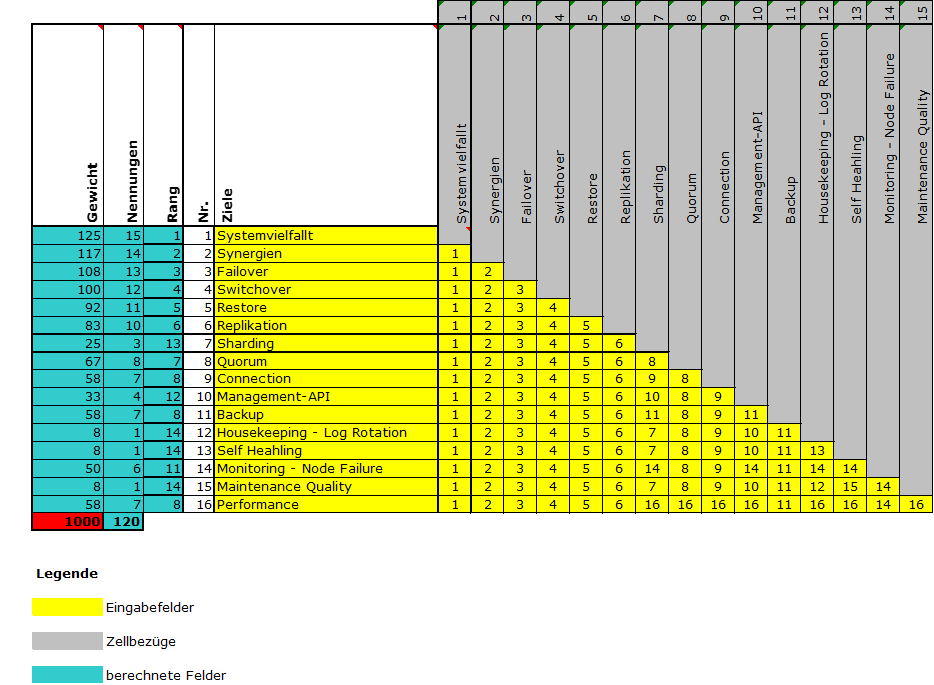
\includegraphics[width=1\linewidth]{source/implementation/evaluation/requirements/preference_matrix}
        \caption{Präferenzmatrix}
        \label{fig:preference_matrix}
    \end{figure}
\end{flushleft}
%\begin{flushleft}
%    Die Gewichtung der Failover-Anforderungen setzt sich wie folgt zusammen:
%    \begin{figure}[H]
%        \centering
%        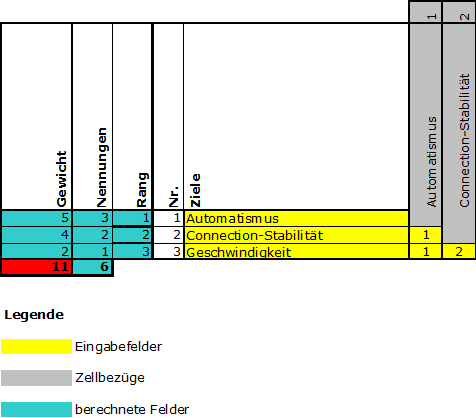
\includegraphics[width=0.75\linewidth]{source/implementation/evaluation/requirements/preference_matrix_failover}
%        \caption{Präferenzmatrix - Failover}
%        \label{fig:preference_matrix_failover}
%    \end{figure}
%\end{flushleft}
%\begin{flushleft}
%    Beim Switchover wurde die Gewichtung wie folgt aufgeteilt:
%    \begin{figure}[H]
%        \centering
%        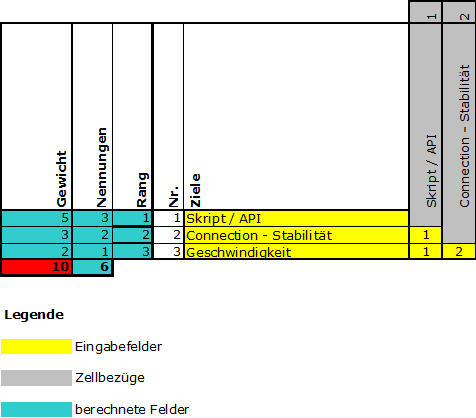
\includegraphics[width=0.75\linewidth]{source/implementation/evaluation/requirements/preference_matrix_switchover}
%        \caption{Präferenzmatrix - Switchover}
%        \label{fig:preference_matrix_switchover}
%    \end{figure}
%\end{flushleft}
%\begin{flushleft}
%    Die Gewichtung und Aufteilung der Restore-Anforderungen sieht wie folgt aus:
%    \begin{figure}[H]
%        \centering
%        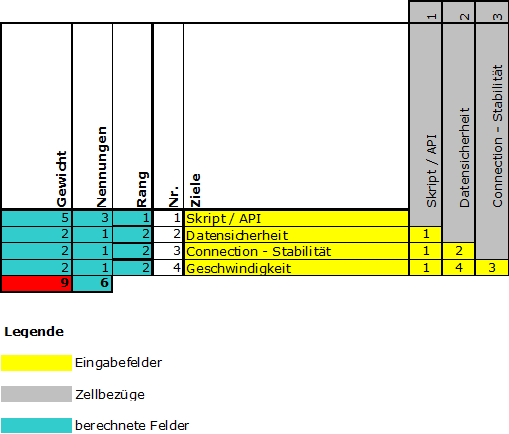
\includegraphics[width=0.75\linewidth]{source/implementation/evaluation/requirements/preference_matrix_restore}
%        \caption{Präferenzmatrix - Restore}
%        \label{fig:preference_matrix_restore}
%    \end{figure}
%\end{flushleft}
%\begin{flushleft}
%    Die Replikationsanforderungen resp.
%    deren Gewichtung ist wie folgt aufgebaut:
%    \begin{figure}[H]
%        \centering
%        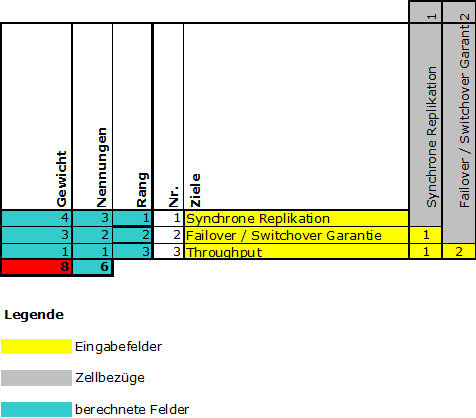
\includegraphics[width=0.75\linewidth]{source/implementation/evaluation/requirements/preference_matrix_replication}
%        \caption{Präferenzmatrix - Replikation}
%        \label{fig:preference_matrix_replication}
%    \end{figure}
%\end{flushleft}
%\begin{flushleft}
%    Das Sharding setzt sich aus folgenden Teilen zusammen:
%    \begin{figure}[H]
%        \centering
%        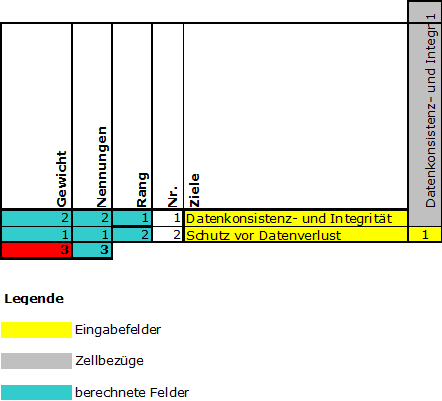
\includegraphics[width=0.75\linewidth]{source/implementation/evaluation/requirements/preference_matrix_sharding}
%        \caption{Präferenzmatrix - Sharding}
%        \label{fig:preference_matrix_sharding}
%    \end{figure}
%\end{flushleft}
%\begin{flushleft}
%    Die Quorum-Anforderung ist folgendermassen zusammengesetzt:
%    \begin{figure}[H]
%        \centering
%        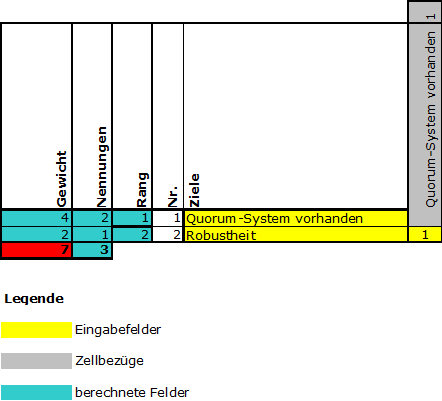
\includegraphics[width=0.75\linewidth]{source/implementation/evaluation/requirements/preference_matrix_quorum}
%        \caption{Präferenzmatrix - Quorum}
%        \label{fig:preference_matrix_quorum}
%    \end{figure}
%\end{flushleft}
%\begin{flushleft}
%    Bei der Management-API gibt es mehrere Sub-Anforderungen:
%    \begin{figure}[H]
%        \centering
%        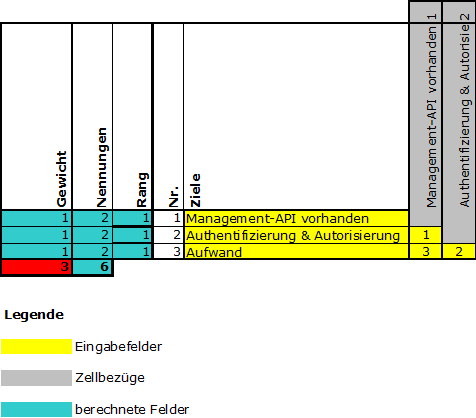
\includegraphics[width=0.75\linewidth]{source/implementation/evaluation/requirements/preference_matrix_management_api}
%        \caption{Präferenzmatrix - Management-API}
%        \label{fig:preference_matrix_management_api}
%    \end{figure}
%\end{flushleft}
%\begin{flushleft}
%    Anforderungen zum Backup wurden nachfolgend aufgeteilt und gewichtet:
%    \begin{figure}[H]
%        \centering
%        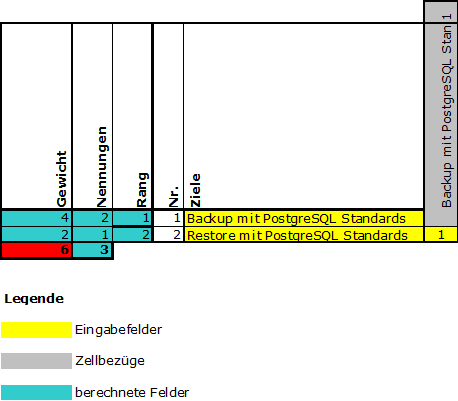
\includegraphics[width=0.75\linewidth]{source/implementation/evaluation/requirements/preference_matrix_backup}
%        \caption{Präferenzmatrix - Backup}
%        \label{fig:preference_matrix_backup}
%    \end{figure}
%\end{flushleft}
%\begin{flushleft}
%    Performance-Benchmarking lässt sich in nachfolgende Teile unterteilen:
%    \begin{figure}[H]
%        \centering
%        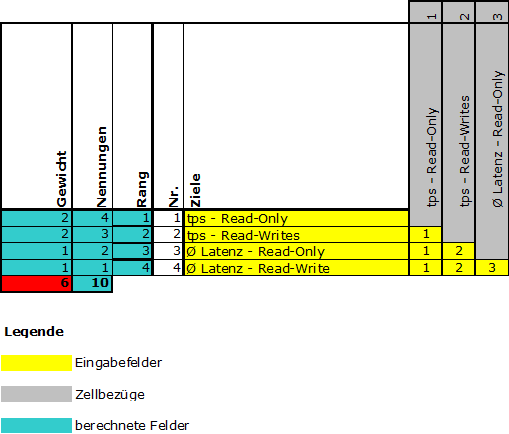
\includegraphics[width=1\linewidth]{source/implementation/evaluation/requirements/preference_matrix_performance}
%        \caption{Präferenzmatrix - Performance}
%        \label{fig:preference_matrix_performance}
%    \end{figure}
%\end{flushleft}
\subsection{Testziele erarbeiten}
\subsection{PostgreSQL Benchmarking}
PostgreSQL bietet ein Benchmarking-Tool,\cite{TYJFF7AB,VXNYQFTE} mit dem die DB Vermessen werden kann.
\subsection{Analyse gängiger PostgreSQL HA Cluster Lösungen}
%! Author = itgramic
%! Date = 05.12.23

% Preamble
\subsubsection{\Gls{PostgreSQL} Replikation}
PostgreSQL bietet von Haus aus Möglichkeiten, um Replikationen durchzuführen.
Dabei ist nicht jede gleich gut für jedes Szenario geeignet\cite{FZAHA89U}.
%! Author = itgramic
%! Date = 05.12.23

% Preamble
\subsubsection{KSGR Lösung}
Das Kantonsspital Graubünden hat basierend auf \gls{keepalived} wird geprüft ob die primäre Seite erreichbar und betriebsbereit ist.
Trifft dies nicht mehr zu, wird ein \Gls{Failover} durchgeführt\cite{NLF2IDBZ}.
Ist die primäre Seite wieder verfügbar, wird ein Restore auf die primäre Seite gefahren.

Es wird beim Restore immer ein komplettes Backup der sekundären Seite auf die primäre Seite übertragen.
Ursache ist, dass die normalerweise für den Datenrestore benötigten \Gls{PostgreSQL} Board mittel nur für eine relativ kurze Zeit eingesetzt werden können ehe die differenzen zwischen den beiden Seiten zu gross werden.

Bei kleinen Datenbanken wie jene für \Gls{Harbor} und \Gls{GitLab} ist die Zeit die hierfür benötigt wird, nicht relevant.
Sind die Datenbanken auf dem \Gls{PostgreSQL Cluster} jedoch grösser, kann der Restore mehrere Minuten dauern.
%! Author = itgramic
%! Date = 05.12.23

% Preamble
\subsubsection{pgpool-II}
\begin{flushleft}
    pgpool-II ist eine Middleware die zwischen einem \Gls{PostgreSQL Cluster} und einem PostgreSQL-Client gesetzt wird.
\end{flushleft}
\begin{flushleft}
    \paragraph{Core-Features}
    pgpool-II bietet folgende Core-Feature\cite{3XWCD3KX}:
    \begin{itemize}
        \item Watchdog für Automatischer Failover
        \item Eigener \Gls{Quorum}-Algorithmus
        \item Integrierter \Gls{Connection Pooler}
        \item Eigenes Replikationssystem
        \item Integriertes Load Balancing
        \item Limiting Exceeding Connections, also queuen von Connections
        \item In Memory Query Caching
        \item Online Node Recovery / Resynchronisation
    \end{itemize}
\end{flushleft}
\begin{flushleft}
    \paragraph{Replikation}
    pgpool-II bietet ein eigenes Replikationssystem an.
\end{flushleft}
\begin{flushleft}
    Es besteht allerdings die Möglichkeit, die PostgreSQL-Standardreplikationen zu verwenden.
\end{flushleft}
\begin{flushleft}
    \paragraph{Proxy}
    pgpool-II hat bereits einen intergrierten Load Balancer.\\
    Einen zusätzlichen Proxy wird daher nicht benötigt.
\end{flushleft}
\begin{flushleft}
    \paragraph{Pooling}
    pgpool-II bietet ebenfalls von Haus aus einen \Gls{Connection Pooler}.
\end{flushleft}
\begin{flushleft}
    \paragraph{API / Skripte}
    pgpool-II bietet mit \texttt{pgpool} ein eigenes Command- und Toolset an.\\
    Mit dem CLI-Tool \texttt{pcp\_command} bietet pgpool-II zudem über eine abgesicherte API,\\
    die auch via Netzwerk erreichbar ist.
\end{flushleft}
\begin{flushleft}
    \paragraph{Maintenance}
    pgpool-II hat kein GitLab- oder GitHub-Repository.
    Metriken wie die GitHub Insights, welche Aufschluss über den Zustand des Projekts geben, finden sich nicht.
\end{flushleft}
\begin{flushleft}
    Die Dokumentation wird zwar aktualisiert, ist aber sehr minimalistisch gehalten.\\
    Sie bietet nur wenig Informationen zum Aufbau und Architektur von pgpool-II.
\end{flushleft}


%! Author = itgramic
%! Date = 05.12.23

% Preamble
\clearpage
\begin{flushleft}
    \subsubsection{pg\_auto\_failover}
    pg\_auto\_failover ist eine PostgreSQL-Erweiterung, die von der Microsoft Subunternehmen Citus Data entwickelt wird.
\end{flushleft}
\begin{flushleft}
    \paragraph{Core-Features}
    Die wichtigsten Features von pg\_auto\_failover sind:
    \begin{itemize}
        \item API
        \item PostgreSQL Extension, also reines PostgreSQL
        \item State Machine Driven
        \item Replikations-Quorum
        \item Citus kompatibel
        \item Azure VM Support
    \end{itemize}
\end{flushleft}
\begin{flushleft}
    \paragraph{Replikation}
    pg\_auto\_failover bietet die Standard PostgreSQL-Replikationen.
\end{flushleft}
\begin{flushleft}
    \paragraph{Proxy}
    pg\_auto\_failover benötigt einen \Gls{HAProxy}, um Load Balancing betreiben zu können  \cite{VYXTI7BS}.
\end{flushleft}
\begin{flushleft}
    \paragraph{API / Skripte}
    pg\_auto\_failover bietet ein eigenes CLI-Tool, \texttt{pg\_autoctl}.
    Dieses stellt Commands für das Einbinden neuer Nodes,
    das Managen von Nodes (Maintenance resp. Switchover),\\
    Konfigurieren oder Monitoren des Systems zur Verfügung \cite{4X2AKDB6}.
\end{flushleft}
\clearpage
\begin{flushleft}
    \paragraph{Architektur}
    Die Dokumentation resp. Grafik von pg\_auto\_failover  \cite{PZZIZ5RT} zeigt auf, wie der Failover funktioniert:
    \begin{figure}[H]
        \centering
        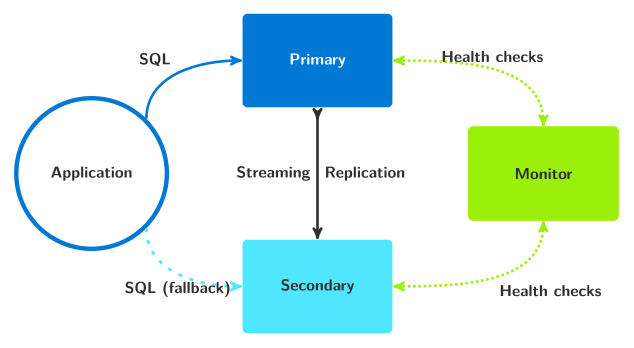
\includegraphics[width=0.75\linewidth]{source/implementation/evaluation/postgresql_ha_solutions/pg_auto_failover/pg_auto-failover_arch-single-standby}
        \caption{pg\_auto\_failover-Architektur - Single Standby}
        \label{fig:pg_auto-failover_arch-single-standby}
    \end{figure}
    Aber wie die Grafik zeigt, können auch Multi-Nodes können eingebunden werden \cite{4ZKBDG57}:
    \begin{figure}[H]
        \centering
        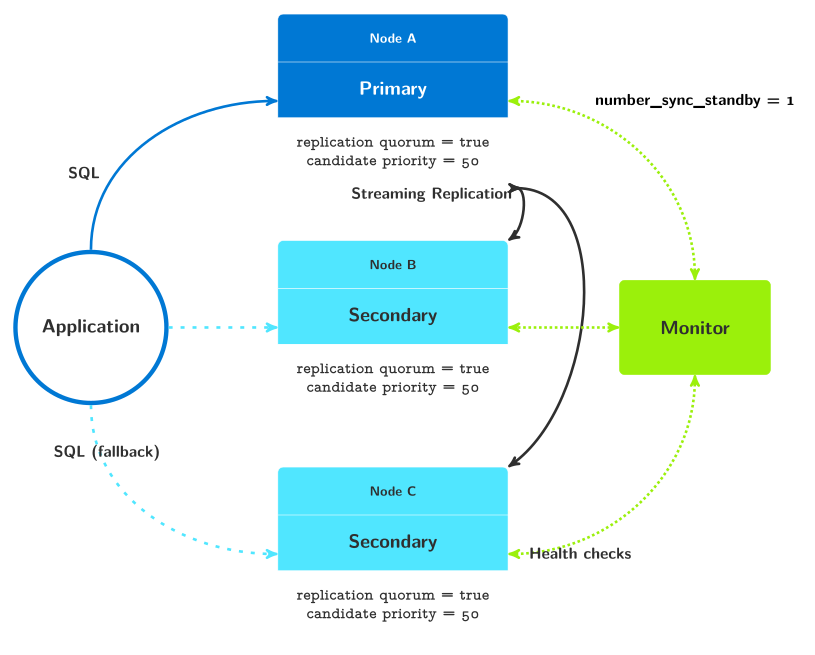
\includegraphics[width=0.75\linewidth]{source/implementation/evaluation/postgresql_ha_solutions/pg_auto_failover/pg_auto-failover_arch-multi-standby}
        \caption{pg\_auto\_failover-Architektur - Multi-Node Standby}
        \label{fig:pg_auto-failover_arch-multi-standby}
    \end{figure}
    \clearpage
    pg\_auto\_failover kann Citus einbinden.
    Allerdings bleibt die Architektur im Kern immer monolithisch.\\
    Die nachfolgende Grafik zeigt die Architektur mit Citus \cite{3FVHLIFE}:
    \begin{figure}[H]
        \centering
        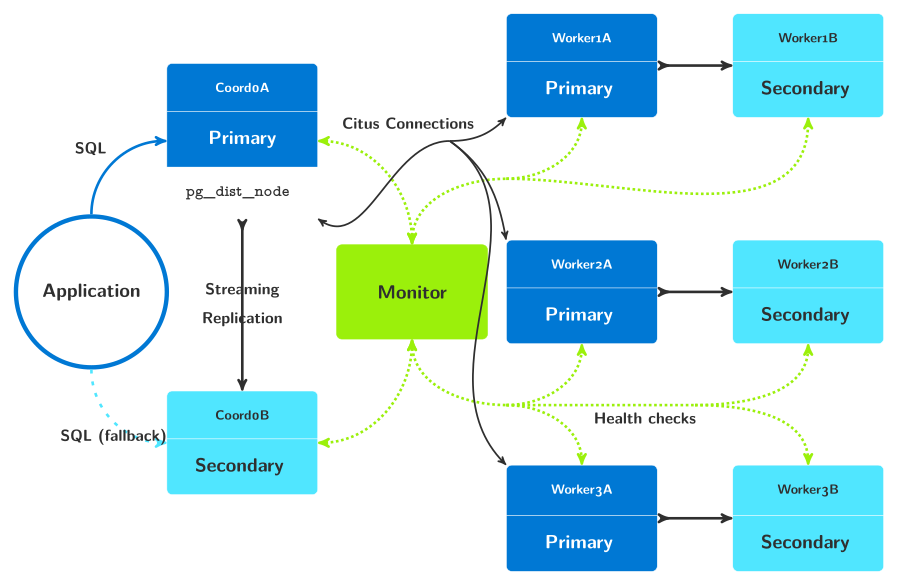
\includegraphics[width=0.75\linewidth]{source/implementation/evaluation/postgresql_ha_solutions/pg_auto_failover/pg_auto-failover_arch-citus}
        \caption{pg\_auto\_failover-Architektur - Citus}
        \label{fig:pg_auto-failover_arch-citus}
    \end{figure}
\end{flushleft}
\begin{flushleft}
    \paragraph{Synergien und Mehrwert}
    pg\_auto\_failover bietet eine Docker-Compose-Integration.\\
    Allerdings ist keine Kubernetes-Integration dokumentiert.
\end{flushleft}
\begin{flushleft}
    Damit bietet pg\_auto\_failover keine Möglichkeit\\
    Synergien zwischen monolithischer Architektur und einer Cloud-Native-Umsetzung auf Kubernetes.\\
    Entsprechend ist kein Mehrwert vorhanden.
\end{flushleft}
%! Author = itgramic
%! Date = 05.12.23

% Preamble
\clearpage
\begin{flushleft}
    \subsubsection{Patroni}
    Patroni ist eine von Zalando auf Basis von Python entwickelte HA-Lösung für \Gls{PostgreSQL}.\\
    Patroni wird aktiv von Zalando gepflegt.
\end{flushleft}
\begin{flushleft}
    \paragraph{Core-Features}
    Patroni bietet folgende Core-Features:
    \begin{itemize}
        \item Rest-API und eigenes Skript- und Toolset
        \item Aktionen und Konfigurationen im Konsensprinzip abgestimmt
        \item Manueller oder Sheduled Switchover
        \item Reines PostgreSQL als Basis, Patroni setzt Hilfe von Python darauf auf
        \item Automatische reintegration von Nodes nach einem Fehler
        \item Citus kompatibel
        \item Docker und Docker-compose Dokumentation
    \end{itemize}
\end{flushleft}
\begin{flushleft}
    \paragraph{Replikation}
    Patroni bietet per Default eine eigene Replikation an.\\
    Diese ist allerdings eine asynchrone Replikation.
\begin{flushleft}
    Patroni unterstützt aber die synchrone Replikation von \Gls{PostgreSQL}.
\end{flushleft}
\end{flushleft}
\begin{flushleft}
    \paragraph{Proxy}
    Patroni benötigt einen \Gls{HAProxy}, um Load Balancing betreiben zu können\cite{VYXTI7BS}.
\end{flushleft}
\begin{flushleft}
    \paragraph{Pooling}
    Patroni benötigt einen externen \Gls{Connection Pooler}.\\
    Hier wird oft PgBouncer \cite{ATBELZ2X} verwendet.
\end{flushleft}
\begin{flushleft}
    \paragraph{API / Skripte}
    Patroni hat ein eigenes Tool- und Commandset, \texttt{patronictl}, welches die Verwaltung vereinfacht.\\
    Es umfasst das Ändern und Erfassen von Konfigurationen, das Forcieren eines Failovers als Switchover, Maintenance Handling und Informationsbeschaffung.\\
    Zusätzlich bietet Patroni eine API, welche Daten für das Monitoring bereitstellt,\\
    aber auch Betriebsfunktionen zur Verfügung stellt.\\
\end{flushleft}
\begin{flushleft}
    \paragraph{\gls{etcd}}
    Patroni benötigt etcd oder \Gls{Consul} als \Gls{Key-Value-Store}.
\end{flushleft}
\begin{flushleft}
    \paragraph{Architektur}
    Das Architektur-Schaubild sieht folgendermassen aus:
    \begin{figure}[H]
        \centering
        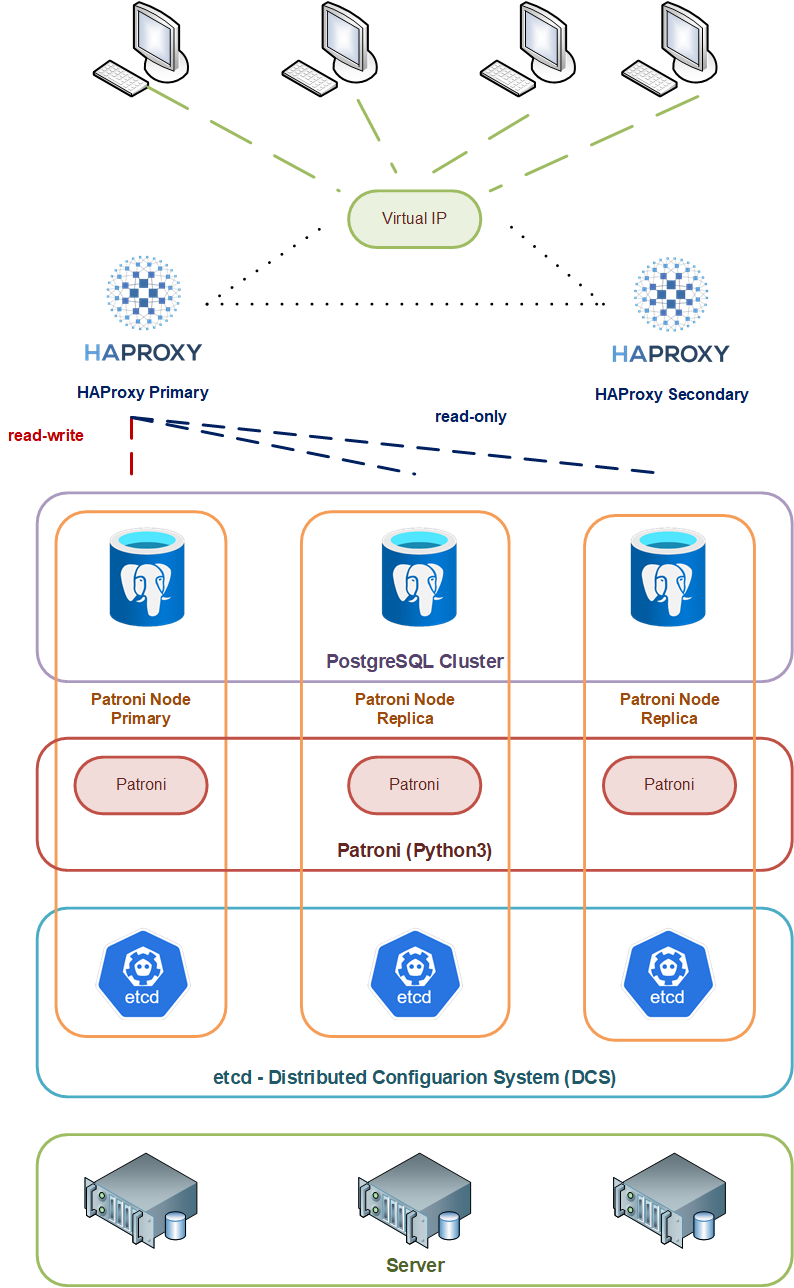
\includegraphics[width=0.7\linewidth]{source/implementation/evaluation/postgresql_ha_solutions/patroni_architecture}
        \caption{Patroni-Architektur}
        \label{fig:patroni-architecture}
    \end{figure}
\end{flushleft}
\begin{flushleft}
    \paragraph{Maintenance}
    Patroni ist ein sehr gepflegtes Projekt, welches die gängigen Community Standards einhält.\\
    Die Details sind im \hyperref[subsec:maintenance_patroni]{Anhang - Maintenance} zu finden.
\end{flushleft}
\begin{flushleft}
    \paragraph{Synergien und Mehrwert}
    Patroni kann nicht nur mit Citus zu einem Distributed / Sharded SQL System umgebaut werden,\\
    es ist auch Kern von StackGres.
\end{flushleft}
\begin{flushleft}
    Damit könnten die API und Skripte in beiden Welten verwendet werden.\\
    Der Aufwand für die Verwaltung und Optimierung würde stark gesenkt.\\
    Projekte wie \texttt{vitabaks / postgresql\_cluster}\cite{HIQVBEPF} bieten zudem die Vorlage für eine noch stärkere Automatisierung.
\end{flushleft}
%! Author = itgramic
%! Date = 05.12.23

% Preamble
\begin{flushleft}
    \subsubsection{CloudNativePG}
    CloudNativePG ist eine Containerlösung für PostgreSQL auf Kubernetes.
\end{flushleft}
\begin{flushleft}
    \paragraph{Core-Features}
    Die wichtigsten Features von CloudNativePG sind\cite{5ALQPE2U}:
    \begin{description}
        \item k8s API integration
        \item Autoamtischer Failover
        \item Self-Healing von Nodes resp. Replikas
        \item Skalierbarkeit (Vertikal, Horizontal bedingt)
        \item Volumne Backup
        \item Object Backup
        \item Rolling PostgreSQL Upgrade / Updates
        \item Pooling mit PgBouncer
        \item Offline und Online Import von bestehenden PostgreSQL DBs
    \end{description}
\end{flushleft}
\begin{flushleft}
    \paragraph{Replikation}
    CloudNativePG bietet die üblichen PostgreSQL Replikaionen an.
\end{flushleft}
\begin{flushleft}
    \paragraph{Proxy}
    CloudNativePG benötigt keinen zusätzlichen Proxy.
\end{flushleft}
\begin{flushleft}
    \paragraph{Pooling}
    CloudNativePG unterstützt pgBouncer als Pooler.
\end{flushleft}
\begin{flushleft}
    \paragraph{API / Skripte}
    CloudNativePG bietet eine API zum Monitoren und Verwalten von Backups, Clustern und dem System selbst\cite{L7PXKAUY}.
\end{flushleft}
\begin{flushleft}
    \paragraph{Architektur}
    Kubernetes regelt die Zugriffe mittels eines entsprechenden Services in die Nodes auf den Pods:
    \begin{figure}[H]
        \centering
        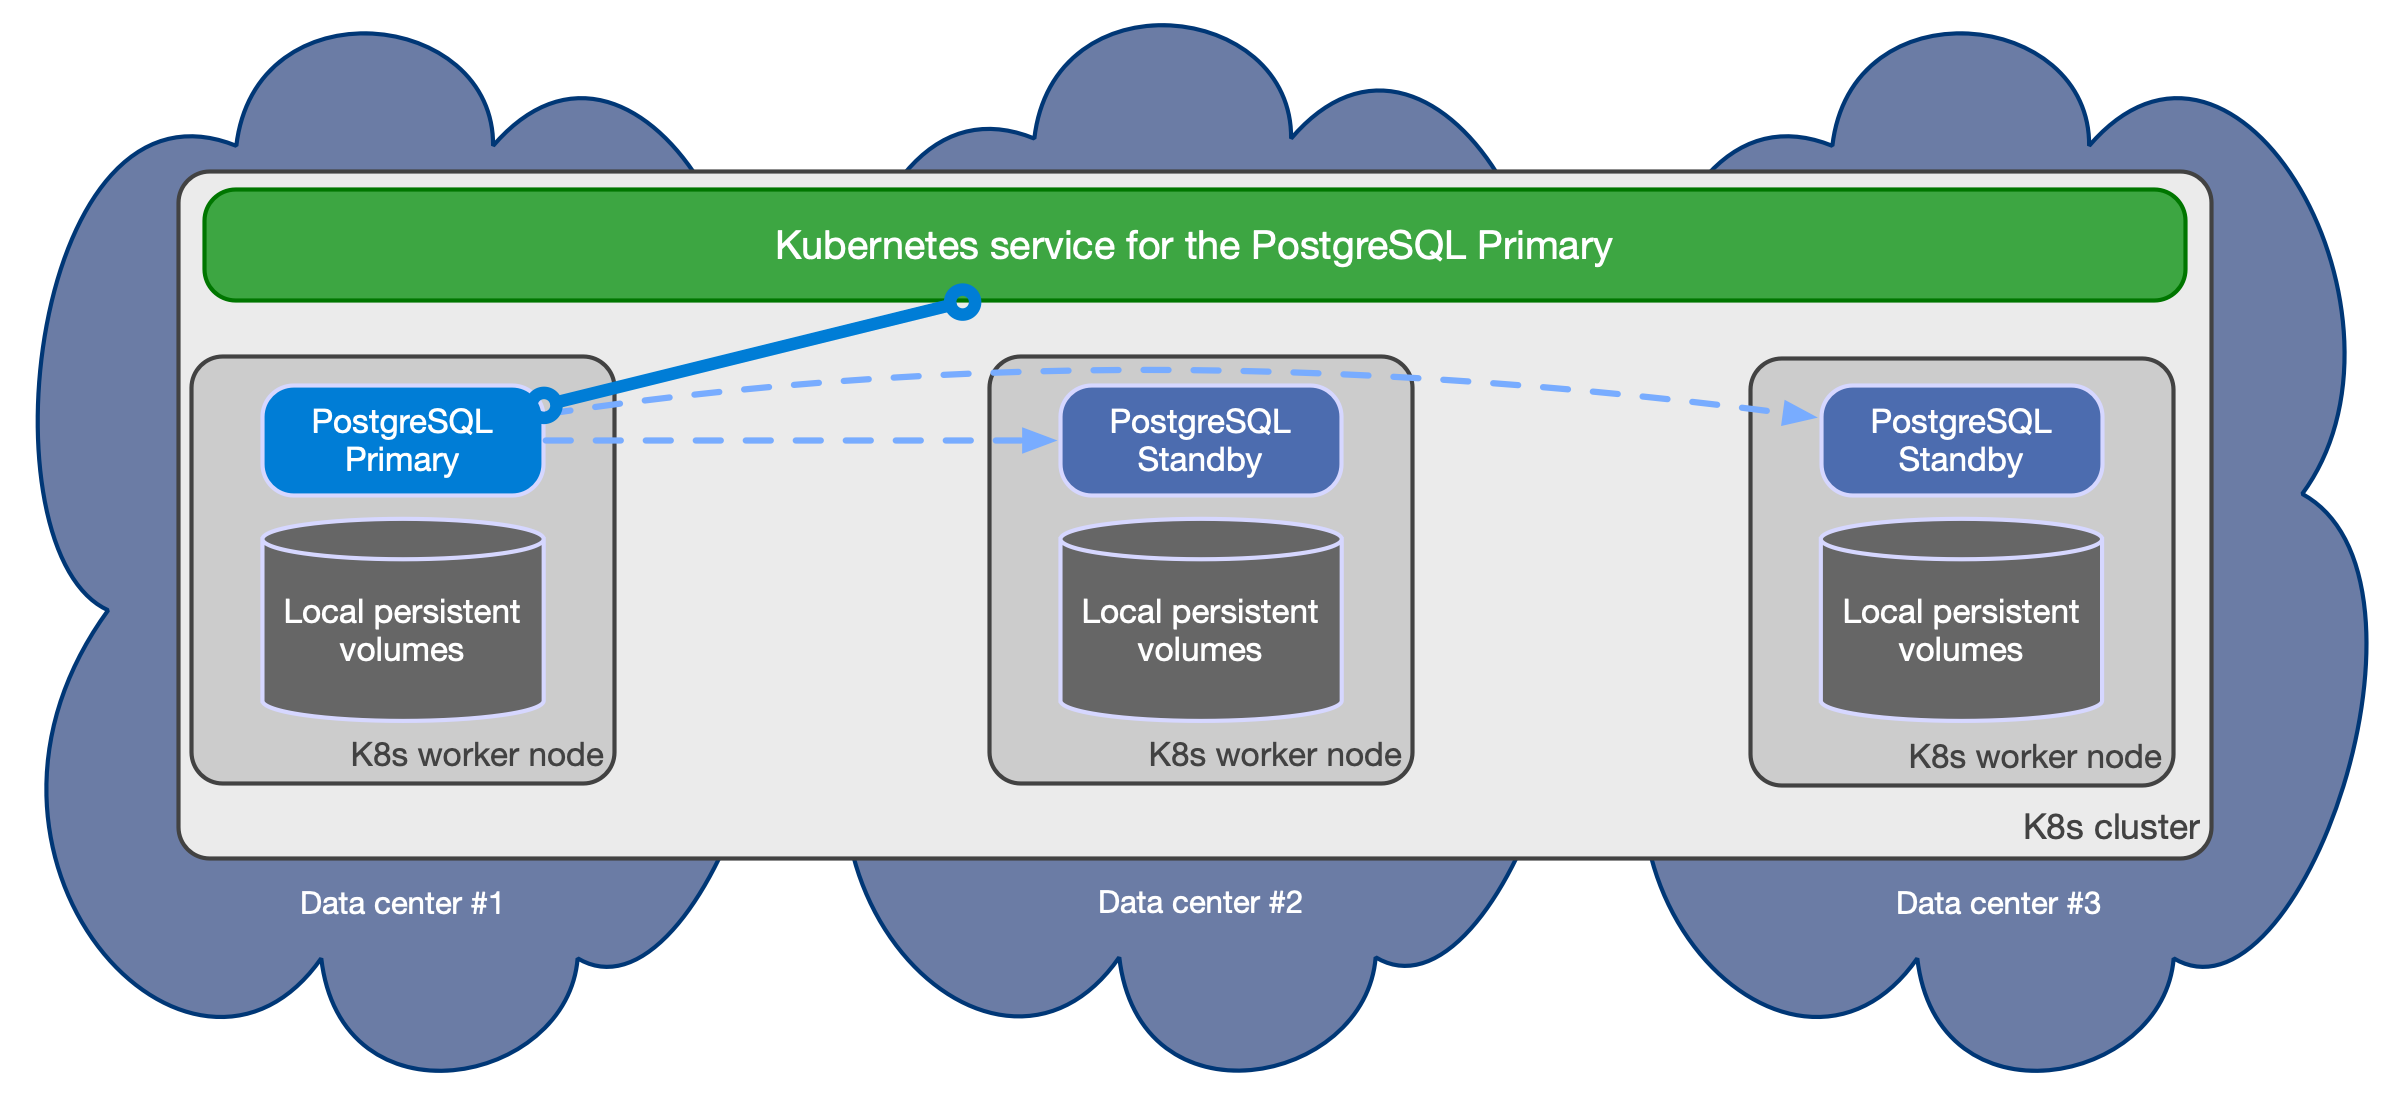
\includegraphics[width=0.75\linewidth]{source/implementation/evaluation/postgresql_ha_solutions/cloudnativepg/k8s-pg-architecture}
        \caption{CloudNativePG - Kubernetes - PostgreSQL}
        \label{fig:k8s-pg-architecture}
    \end{figure}
\end{flushleft}
\begin{flushleft}
    Dabei werden die Read-write workloads an den Primary Node gesendet:
    \begin{figure}[H]
        \centering
        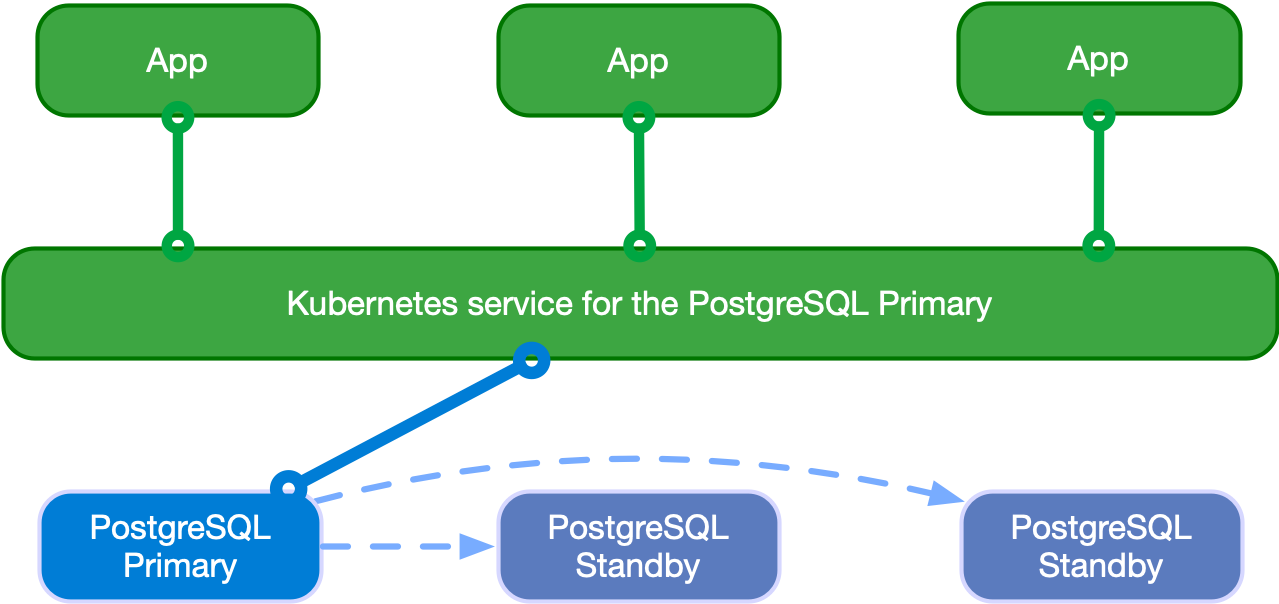
\includegraphics[width=0.75\linewidth]{source/implementation/evaluation/postgresql_ha_solutions/cloudnativepg/cloudnativepg-architecture-rw}
        \caption{CloudNativePG - Kubernetes - Read-write workloads}
        \label{fig:cloudnativepg-architecture-rw}
    \end{figure}
\end{flushleft}
\begin{flushleft}
    Read-only workloads werden mit Round robin an die Replikas zugewiesen:
    \begin{figure}[H]
        \centering
        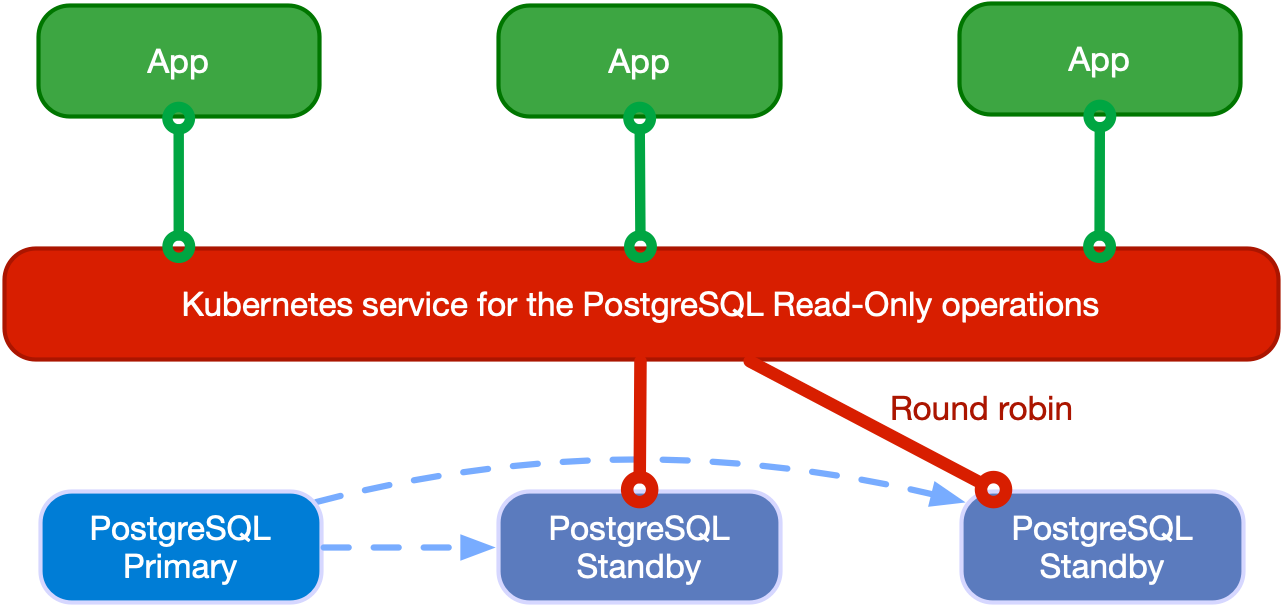
\includegraphics[width=0.75\linewidth]{source/implementation/evaluation/postgresql_ha_solutions/cloudnativepg/cloudnativepg-architecture-read-only}
        \caption{CloudNativePG - Kubernetes - Read-only workloads}
        \label{fig:cloudnativepg-architecture-read-only}
    \end{figure}
\end{flushleft}
\begin{flushleft}
    Es könnten auch Lösungen mit Designated Kubernetes-Clustern in einem anderen RZ oder einer anderen Geo-Region relaisiert werden.
\end{flushleft}
\begin{flushleft}
    \paragraph{Maintenance}
\end{flushleft}
\begin{flushleft}
    \paragraph{Synergien und Mehrwert}
    CloudNativePG bleibt ein Monolithisches System,\\welches aber keine Möglichkeit bietet,\\auch auf einem Normalen Serversetting betrieben zu werden.
\end{flushleft}
\begin{flushleft}
    Daher bietet CloudNativePG weder einen Benefit durch seine Architektur noch mit der Möglichkeit,\\Synergien nutzen zu können.
\end{flushleft}
%! Author = gramic
%! Date = 22.04.24

% Preamble
\begin{flushleft}
    \subsection{YugabyteDB}
    \label{subsec:appendix_testing_yugabytedb}
    Zum einen kann der Fehler irgendwann auftreten.\\
    In diesem Fall wird erst im Log die Fehlermeldung geworfen, dass die Zeitdifferenz zu gross ist:
    \begin{figure}[H]
        \centering
        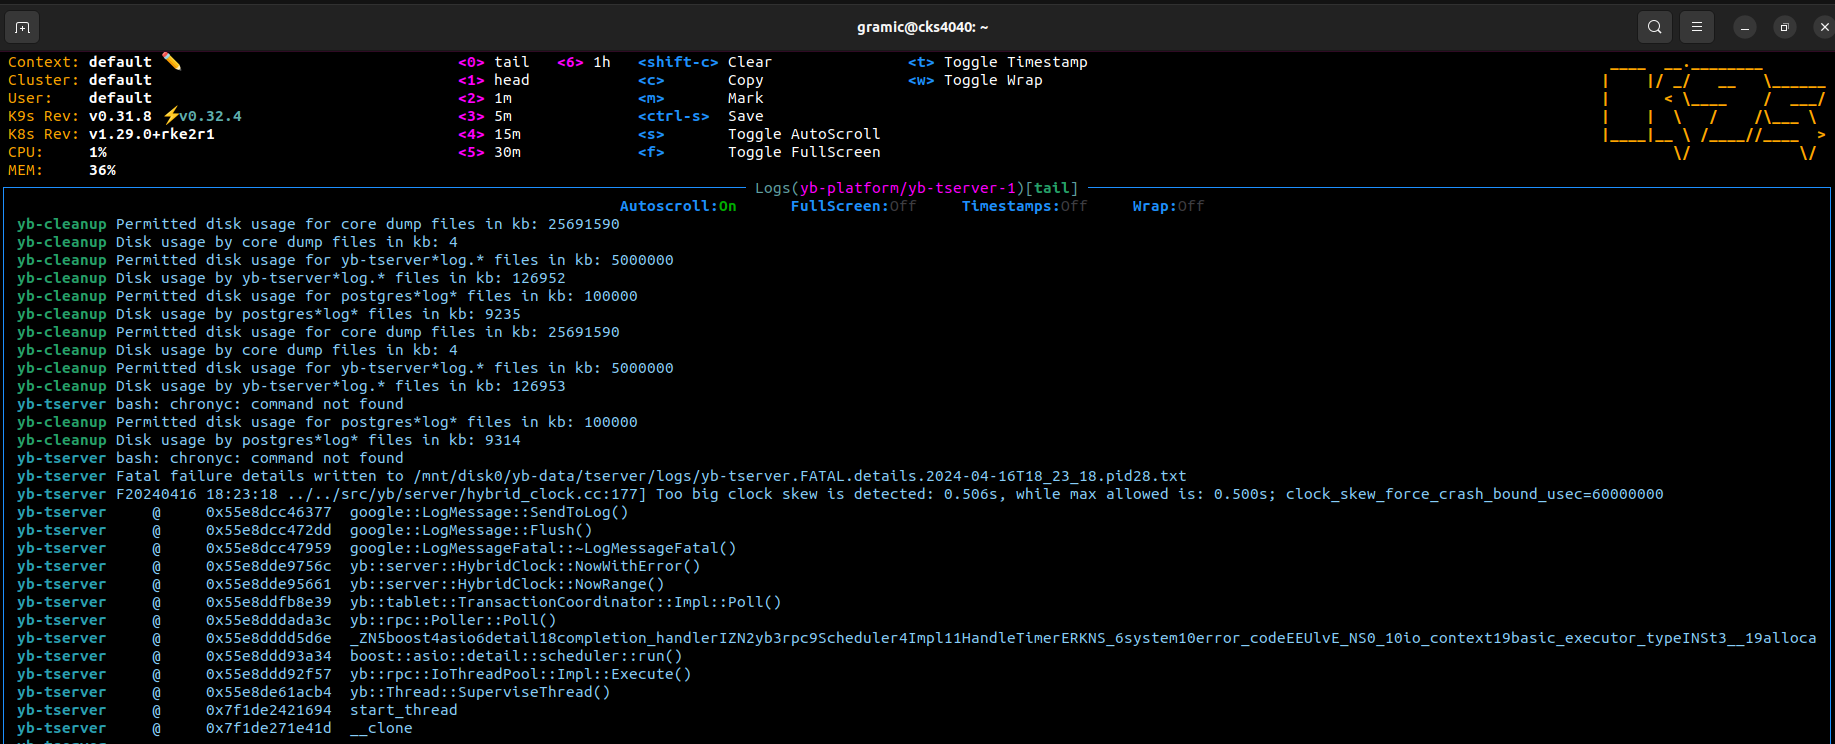
\includegraphics[width=1\linewidth]{source/appendix/evaluation_testing/yugabytedb_too_big_clock_skew_is_detected}
        \caption{YugabyteDB - Too big clock skew is detected}
        \label{fig:yugabytedb_too_big_clock_skew_is_detected}
    \end{figure}
    Eine Folge ist, dass kein neuer Leader bestimmt werden kann:
    \begin{figure}[H]
        \centering
        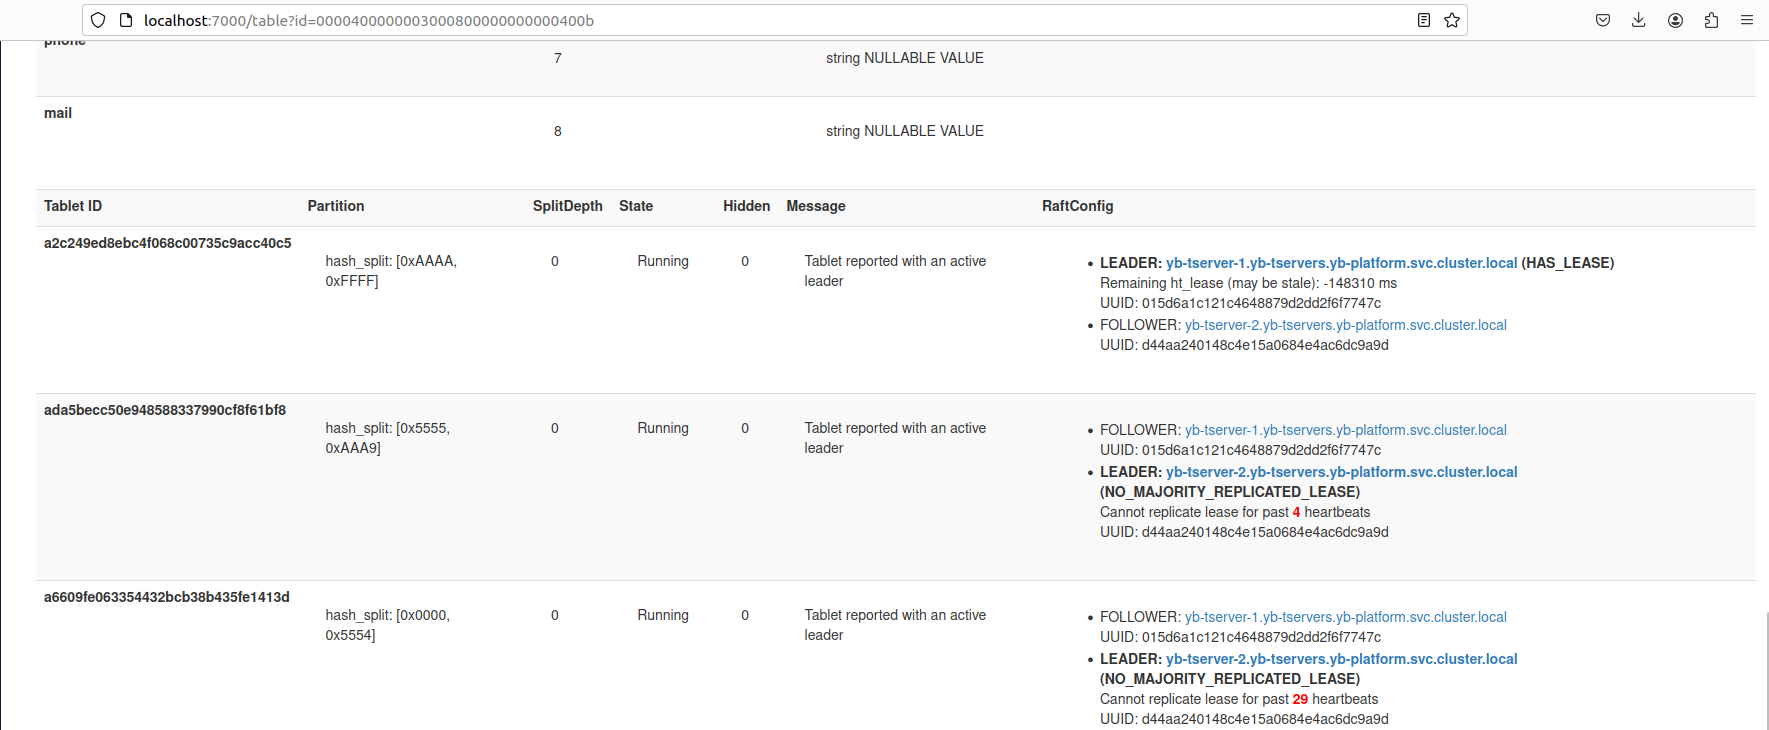
\includegraphics[width=1\linewidth]{source/appendix/evaluation_testing/yugabytedb_tablet_leader_lease}
        \caption{YugabyteDB - Tablet Leader - No Lease}
        \label{fig:yugabytedb_tablet_leader_lease}
    \end{figure}
    Als nächstes wird der komplette \texttt{tserver} in einem \texttt{CrashLoopBackOff} fallen:
    \begin{figure}[H]
        \centering
        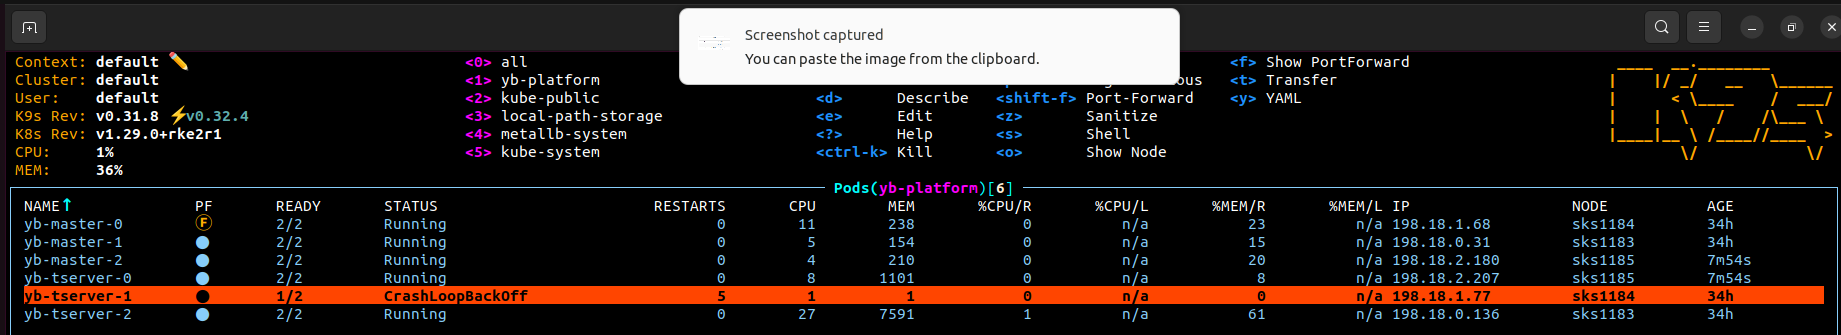
\includegraphics[width=1\linewidth]{source/appendix/evaluation_testing/yugabytedb_crashloopbackoff}
        \caption{YugabyteDB - CrashLoopBackOff}
        \label{fig:yugabytedb_crashloopbackoff}
    \end{figure}
    Der ganze Cluster an sich aber bleibt arbeitsfähig.
\end{flushleft}
\begin{flushleft}
    Anders sieht es aus, wenn auch \texttt{tmaster}-Nodes von Start weg betroffen sind.\\
    Es werden aber primär nur die Logs überall geschrieben:
    \begin{figure}[H]
        \centering
        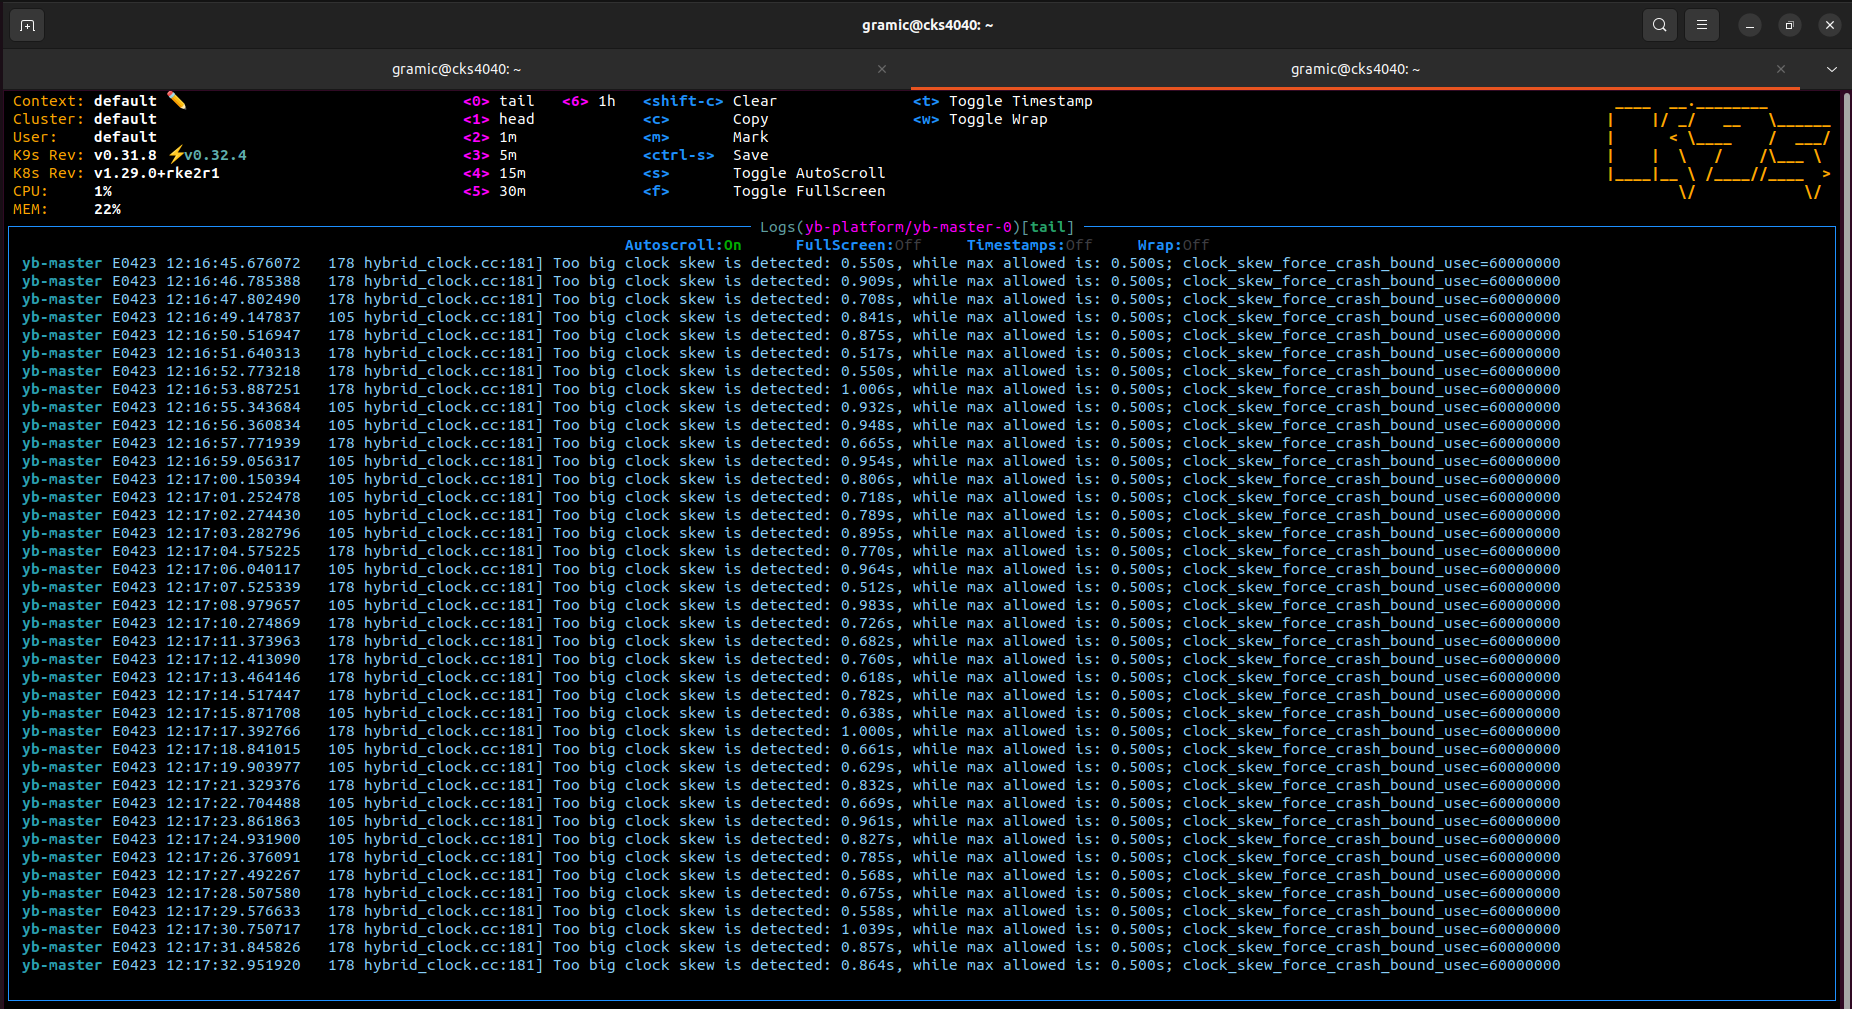
\includegraphics[width=1\linewidth]{source/appendix/evaluation_testing/yugabytedb_yb-tmaster-0_sks1184_clock_error}
        \caption{YugabyteDB - Too big clock skew is detected - tmaster}
        \label{fig:yugabytedb_yb-tmaster-0_sks1184_clock_error}
    \end{figure}
    \begin{figure}[H]
        \centering
        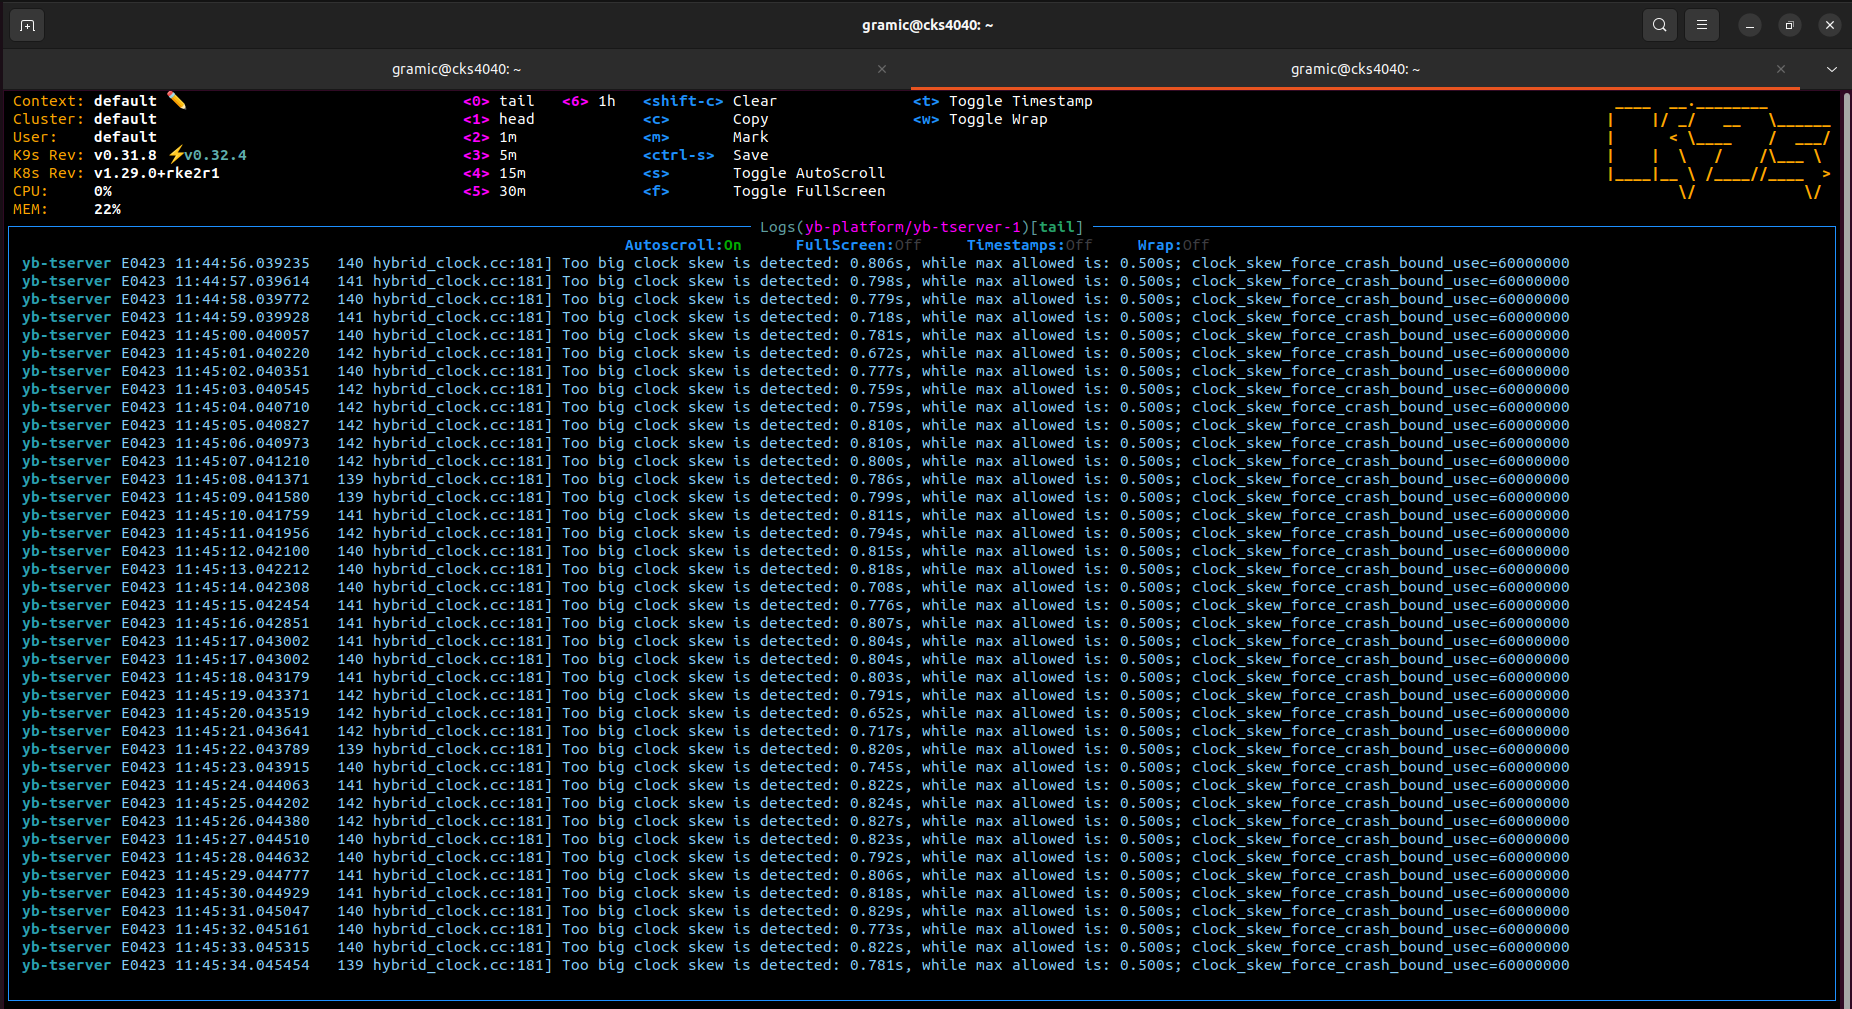
\includegraphics[width=1\linewidth]{source/appendix/evaluation_testing/yugabytedb_yb-tserver-1_sks1184_clock_error}
        \caption{YugabyteDB - Too big clock skew is detected - tserver}
        \label{fig:yugabytedb_yb-tserver-1_sks1184_clock_error}
    \end{figure}
%    \begin{figure}[H]
%        \centering
%        \subfloat[yb-tmaster-0]{{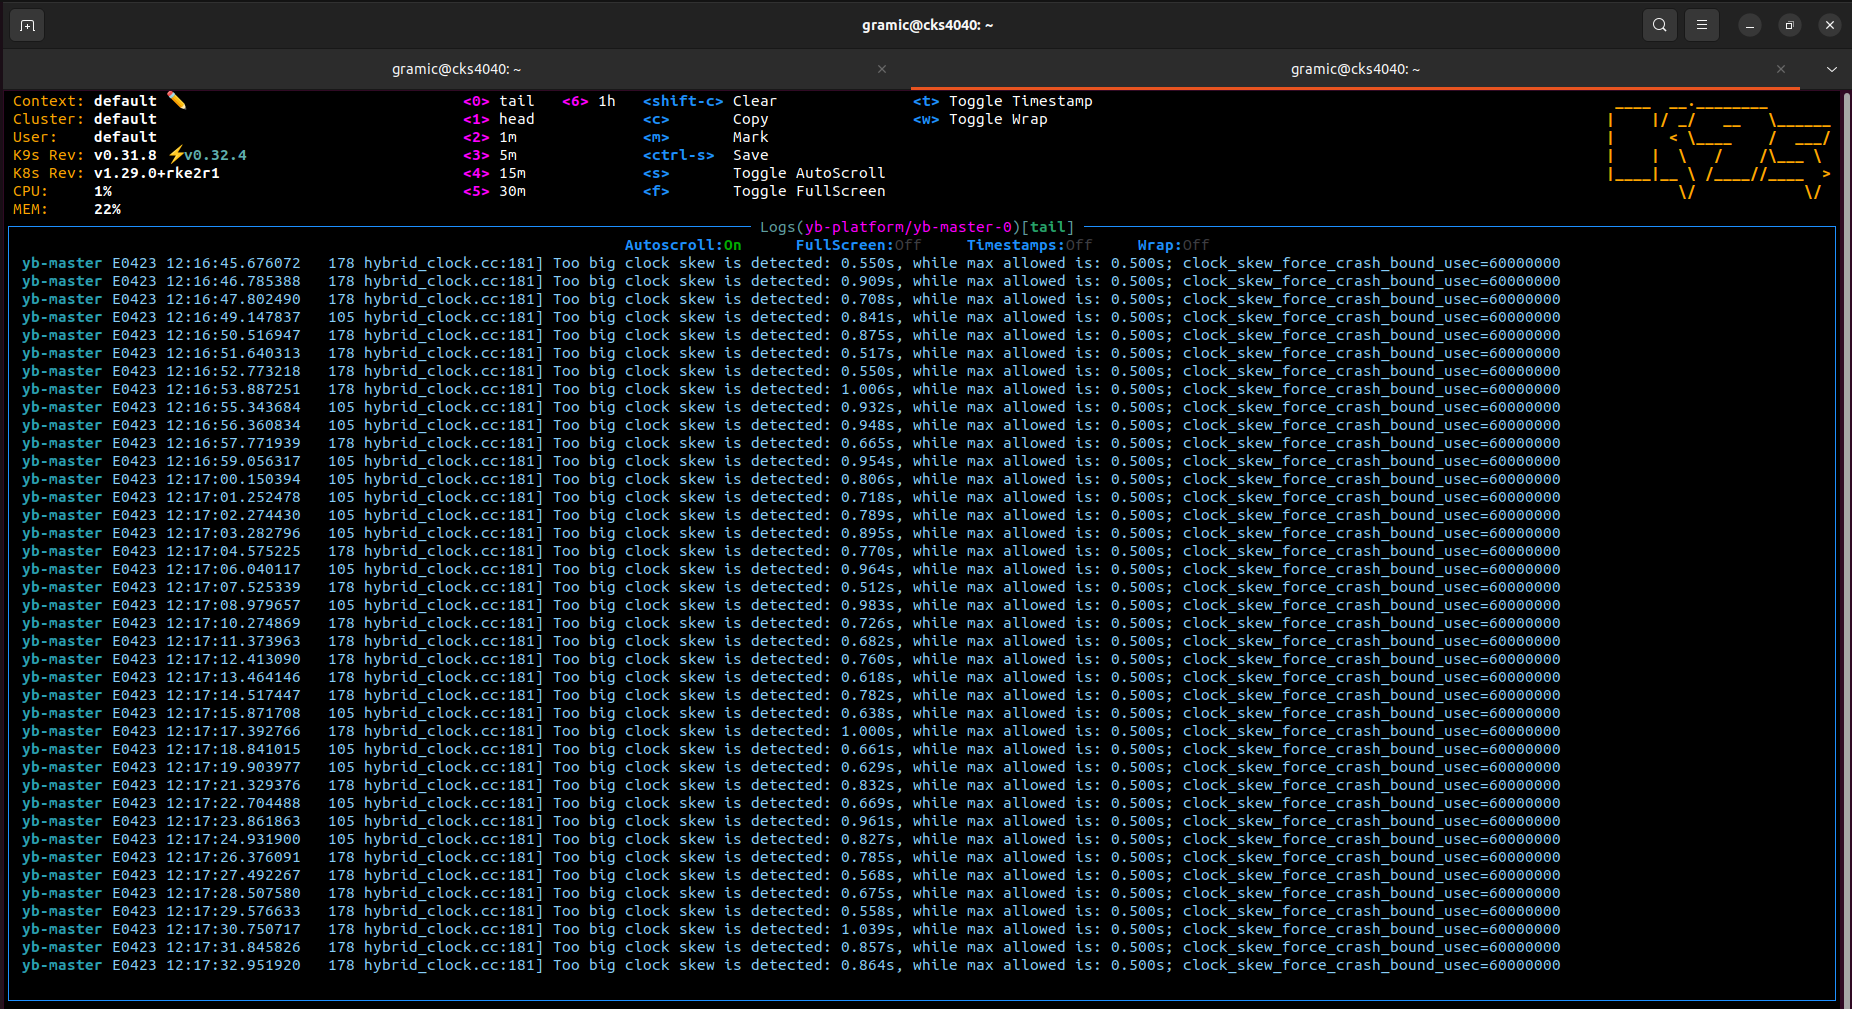
\includegraphics[width=0.47\linewidth]{source/appendix/evaluation_testing/yugabytedb_yb-tmaster-0_sks1184_clock_error} }}%
%        \qquad
%        \subfloat[yb-tserver-1]{{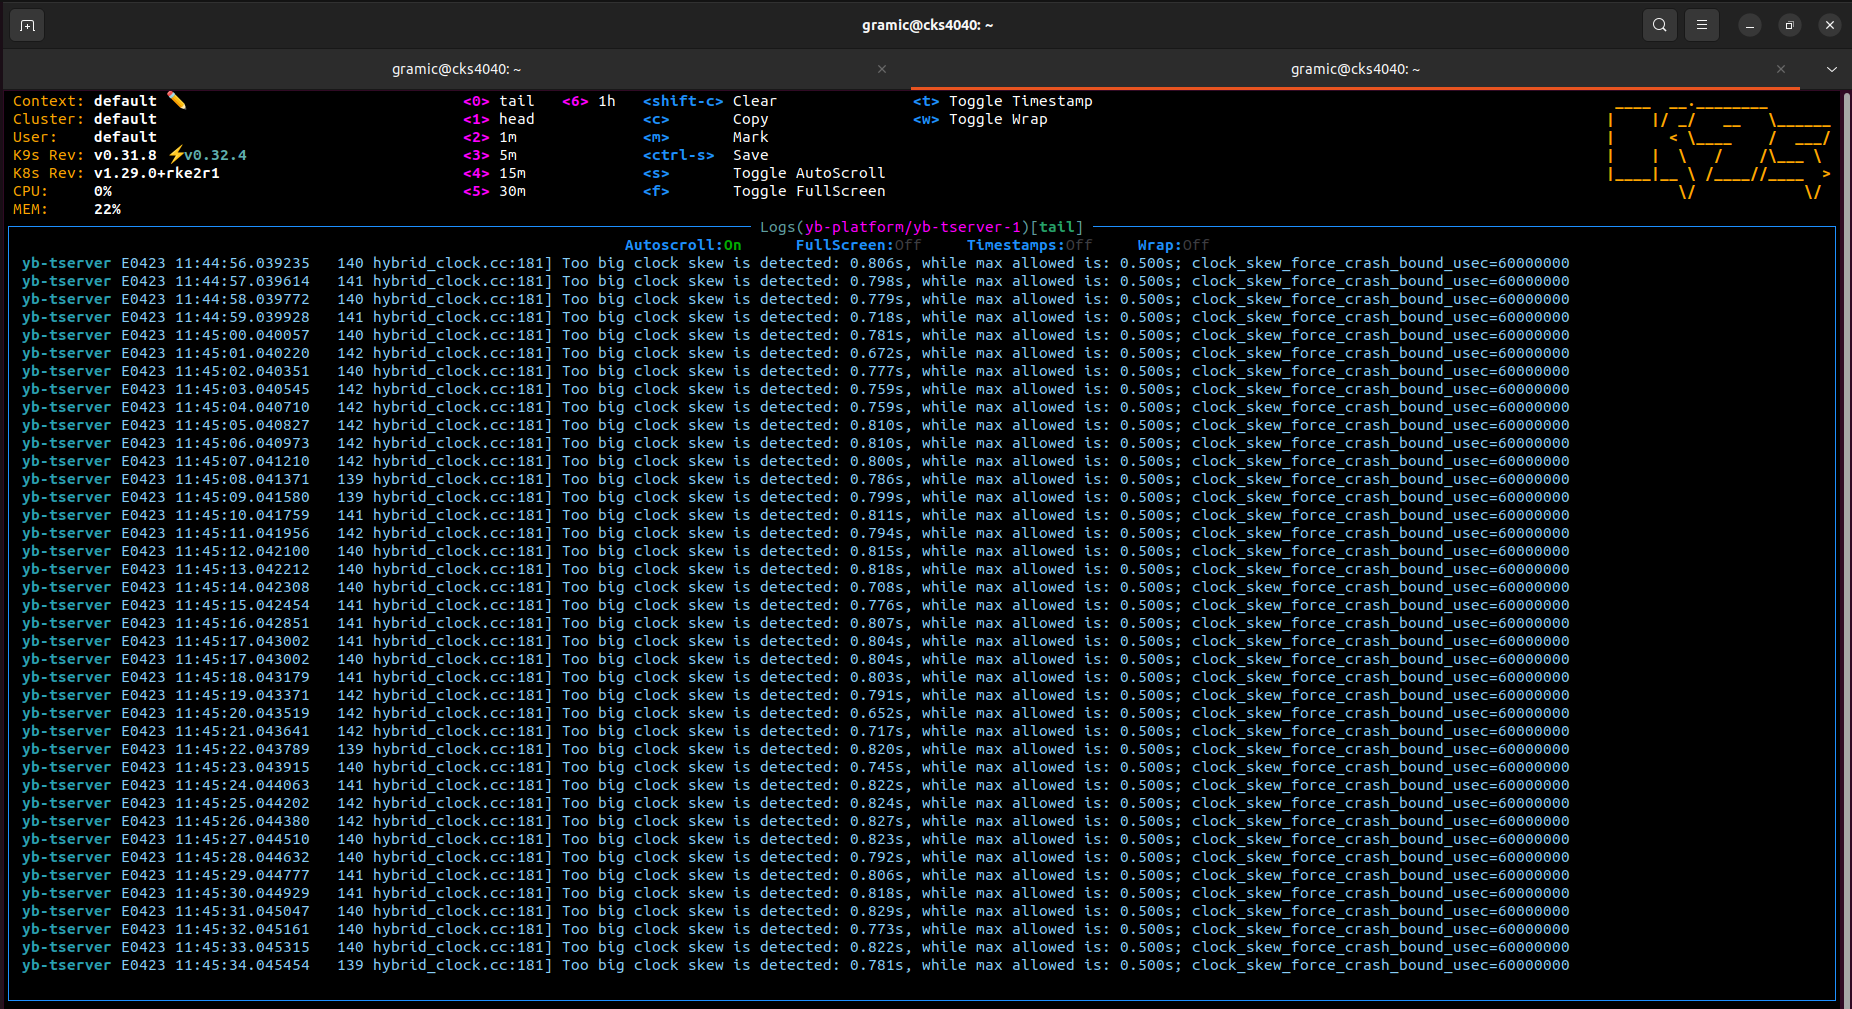
\includegraphics[width=0.47\linewidth]{source/appendix/evaluation_testing/yugabytedb_yb-tserver-1_sks1184_clock_error} }}%
%        \caption{YugabyteDB - Too big clock skew is detected - Node}
%        \label{fig:yugabytedb_sks1184_clock_error}
%    \end{figure}
    YugabyteDB erlaubt in so einem Fall keine Zugriffe mehr auf den Cluster.\\
    So wird verhindert, dass der Cluster korrumpiert wird.
\end{flushleft}
\subsubsection{Stackgres mit Citus}
\begin{flushleft} 
Stackgres ist eine PostgreSQL Implementation die dafür vorgesehenen ist, in einem Kubernetes Cluster betrieben zu werden.
\end{flushleft} 
\begin{flushleft}
An sich wäre Stackgres nur eine Implementation von Patroni in Kubernetes inkl. Load Balancer.\\
Nun kommt das Citus-Plugin ins spiel, welches aus einer jeden Monolithischen, Klassischen PostgreSQL Installation eine Distributed SQL Umgebung macht.////
Citus wiederum ist in den Microsoft Konzern eingebettet
\end{flushleft}

\begin{flushleft}
    \paragraph{Architektur}
    \begin{flushleft}
        \subparagraph{Citus Coordinator und Workers}
        \begin{figure}[H]
            \centering
            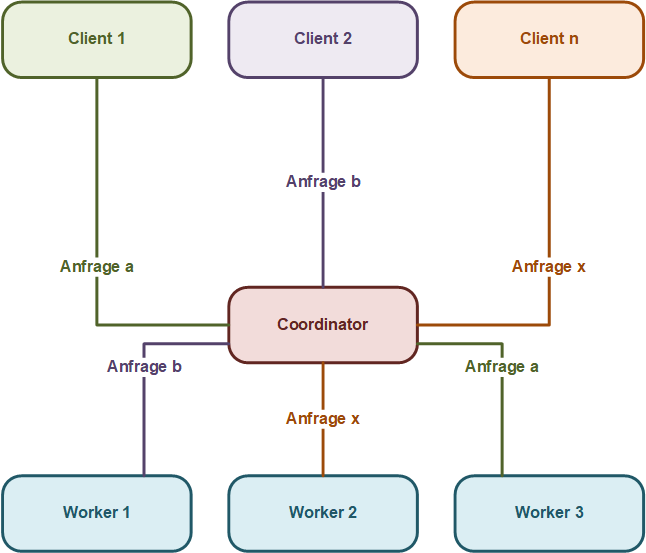
\includegraphics[width=0.75\linewidth]{source/implementation/evaluation/postgresql_ha_solutions/stackgres/citus_coordinator_worker}
            \caption{Citus - Coordinator und Workers}
            \label{fig:citus_coordinator_worker}
        \end{figure}
    \end{flushleft}
    \begin{flushleft}
        \subparagraph{Citus Sharding}
        Citus bietet zwei Sharding-Modelle an.
        \begin{flushleft}
            \textbf{Row-based sharding}
            Beim diesen sharding werden Tabellen anhand einer Distribution Column aufgeteilt. \cite{2Y5FA36C, FDUUL9IM}
        \end{flushleft}
        \begin{flushleft}
            \textbf{Schema-based sharding}
        \end{flushleft}
    \end{flushleft}
\end{flushleft}
\begin{flushleft}
    \paragraph{Maintenance}
    Bei Stackgres gab es im letzten Monat keine wirkliche Bewegung:
    \begin{figure}[H]
        \centering
        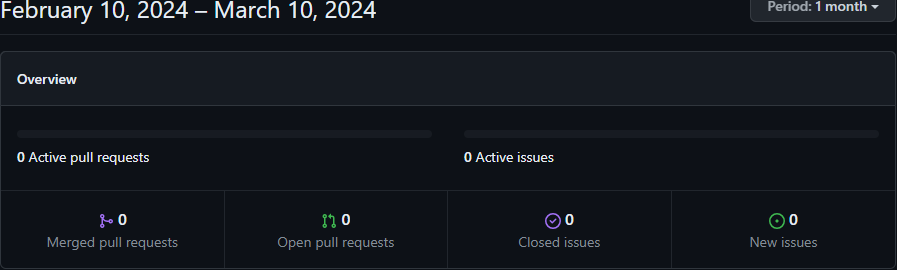
\includegraphics[width=0.75\linewidth]{source/implementation/evaluation/postgresql_ha_solutions/insights/stackgres_citus/pulse_ongres_stackgres}
        \caption{Stackgres - Pulse}
        \label{fig:pulse_ongres_stackgres}
    \end{figure}
    Anders sieht es bei Citus aus, die Firma die mittlerweile zu Microsoft gehört, schliesst Issues rasch und hat eine verhältnissmässig hohe Requstrate:
    \begin{figure}[H]
        \centering
        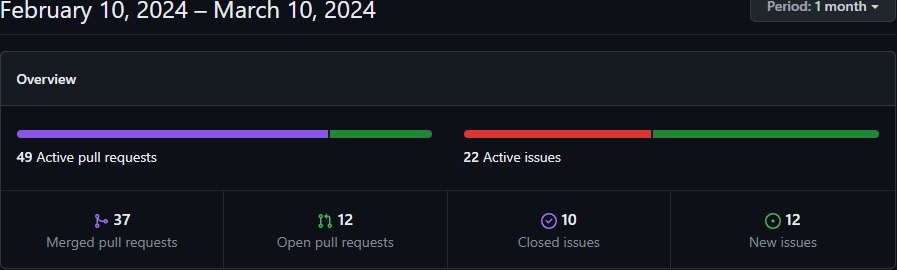
\includegraphics[width=0.75\linewidth]{source/implementation/evaluation/postgresql_ha_solutions/insights/stackgres_citus/pulse_citusdata_citus}
        \caption{Citus - Pulse}
        \label{fig:pulse_citusdata_citus}
    \end{figure}

    Bei Stackgres wird sehr viel Code hinzugefügt oder gelöscht, beim älteren Citus wurden weniger änderungen verzeichnet:
    \begin{figure}[H]
        \centering
        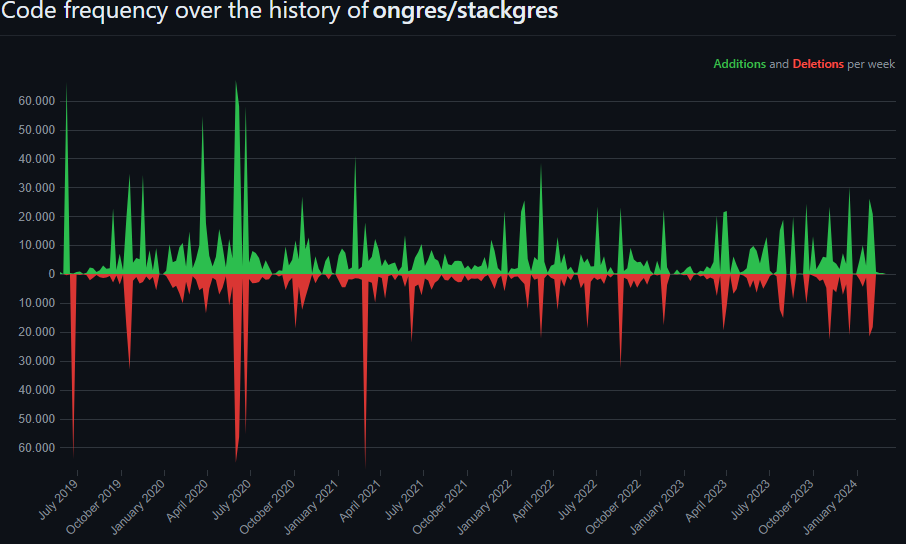
\includegraphics[width=0.75\linewidth]{source/implementation/evaluation/postgresql_ha_solutions/insights/stackgres_citus/code_frequency_ongres_stackgres}
        \caption{Stackgres - Code Frequency}
        \label{fig:code_frequency_ongres_stackgres}
    \end{figure}
    \begin{figure}[H]
        \centering
        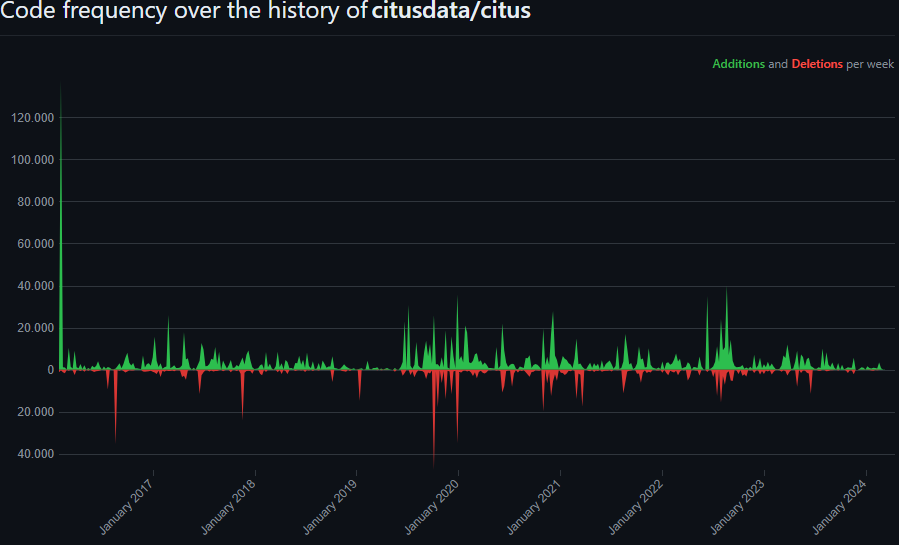
\includegraphics[width=0.75\linewidth]{source/implementation/evaluation/postgresql_ha_solutions/insights/stackgres_citus/code_frequency_citusdata_citus}
        \caption{Citus - Code Frequency}
        \label{fig:code_frequency_citusdata_citus}
    \end{figure}

    Citus legt einen hohen Stellenwert auf die Community-Standars, Stackgres selbst schneidet hier nur Mittelmässig ab:
    \begin{figure}[H]
        \centering
        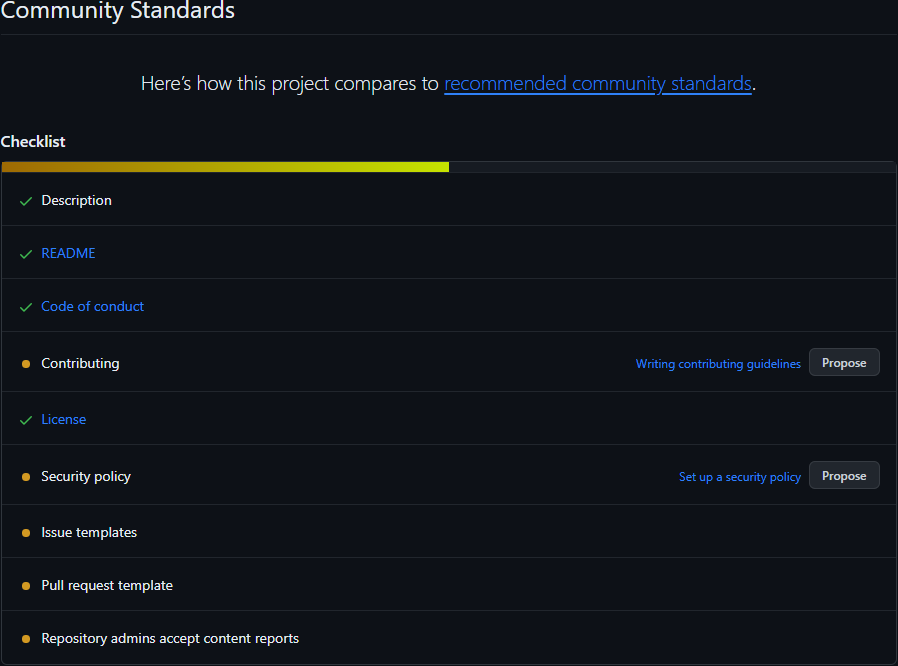
\includegraphics[width=0.75\linewidth]{source/implementation/evaluation/postgresql_ha_solutions/insights/stackgres_citus/stackgres_community_standards}
        \caption{Stackgres - Community Standards}
        \label{fig:stackgres_community_standards}
    \end{figure}
    \begin{figure}[H]
        \centering
        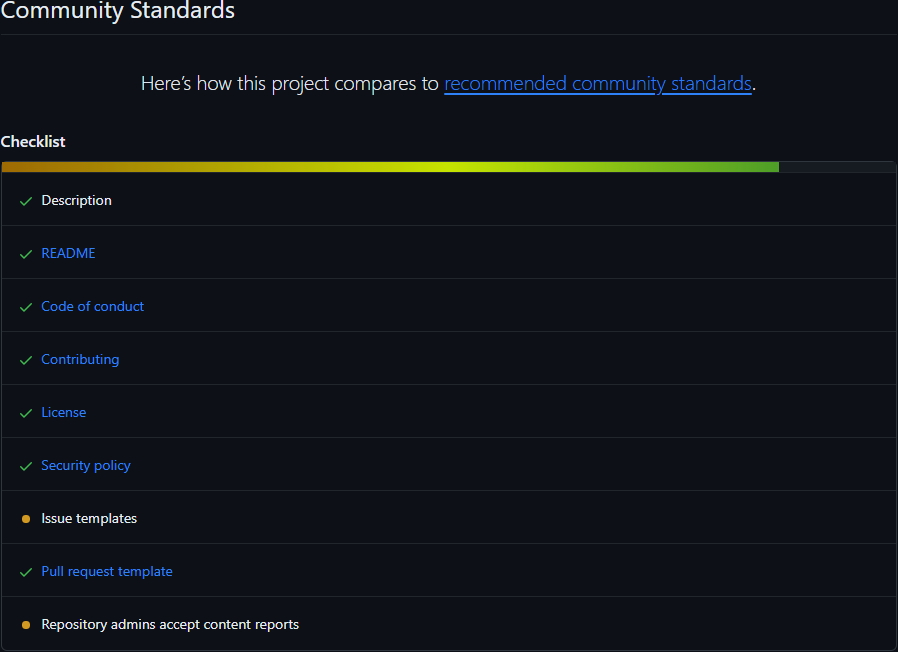
\includegraphics[width=0.75\linewidth]{source/implementation/evaluation/postgresql_ha_solutions/insights/stackgres_citus/citus_community_standards}
        \caption{Citus - Community Standards}
        \label{fig:citus_community_standards}
    \end{figure}

    Die Stackgres Constributors pflegen aktiv Additions ein, löschen Regelmässig und Commiten ebenfalls auf die main-Branch.
    Citus, dessen Repository länger Commited wird, hat weniger bewegung auf die main-Branch.
    \begin{figure}[H]
        \centering
        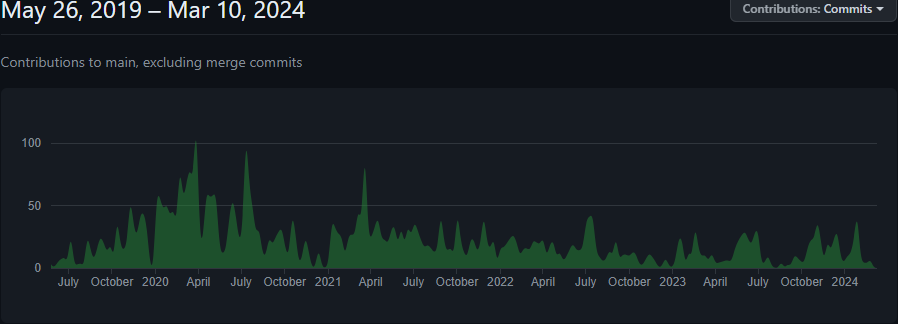
\includegraphics[width=0.75\linewidth]{source/implementation/evaluation/postgresql_ha_solutions/insights/stackgres_citus/contributors_commits_ongres_stackgres}
        \caption{Stackgres - Contributors Commits}
        \label{fig:contributors_commits_ongres_stackgres}
    \end{figure}
    \begin{figure}[H]
        \centering
        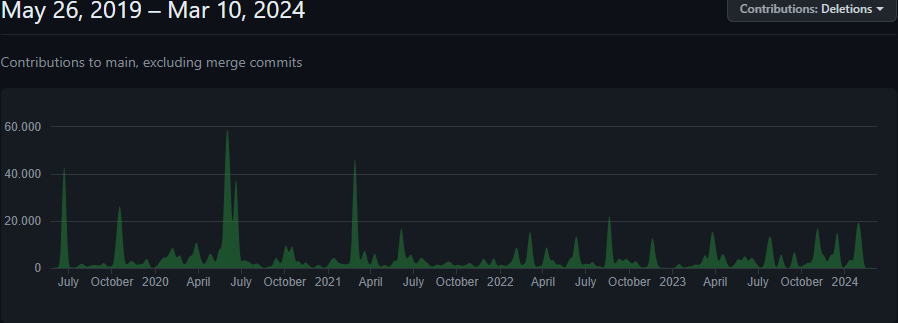
\includegraphics[width=0.75\linewidth]{source/implementation/evaluation/postgresql_ha_solutions/insights/stackgres_citus/contributors_deletations_ongres_stackgres}
        \caption{Stackgres - Contributors Deletations}
        \label{fig:contributors_deletations_ongres_stackgres}
    \end{figure}
    \begin{figure}[H]
        \centering
        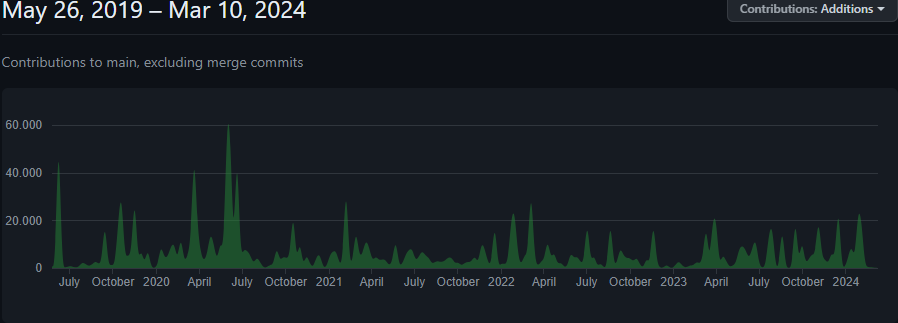
\includegraphics[width=0.75\linewidth]{source/implementation/evaluation/postgresql_ha_solutions/insights/stackgres_citus/contributors_addition_ongres_stackgres}
        \caption{Stackgres - Contributors Additions}
        \label{fig:contributors_addition_ongres_stackgres}
    \end{figure}
    \begin{figure}[H]
        \centering
        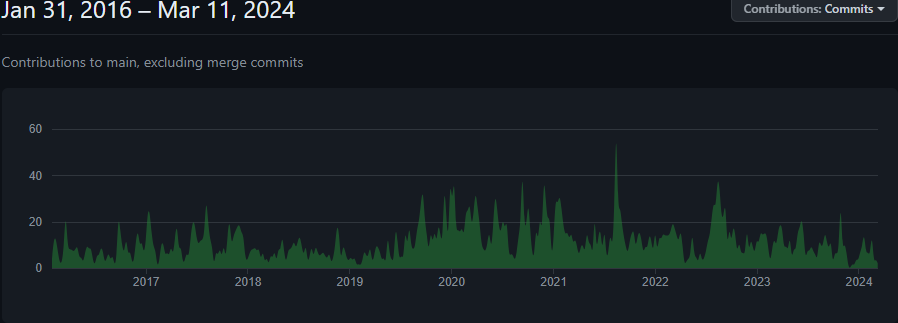
\includegraphics[width=0.75\linewidth]{source/implementation/evaluation/postgresql_ha_solutions/insights/stackgres_citus/contributors_commits_citusdata_citus}
        \caption{Citus - Contributors Commits}
        \label{fig:contributors_commits_citusdata_citus}
    \end{figure}
    \begin{figure}[H]
        \centering
        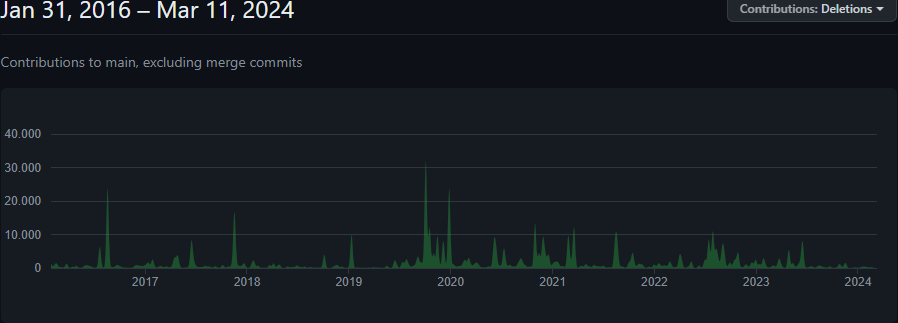
\includegraphics[width=0.75\linewidth]{source/implementation/evaluation/postgresql_ha_solutions/insights/stackgres_citus/contributors_deletations_citusdata_citus}
        \caption{Citus - Contributors Deletations}
        \label{fig:contributors_deletations_citusdata_citus}
    \end{figure}
    \begin{figure}[H]
        \centering
        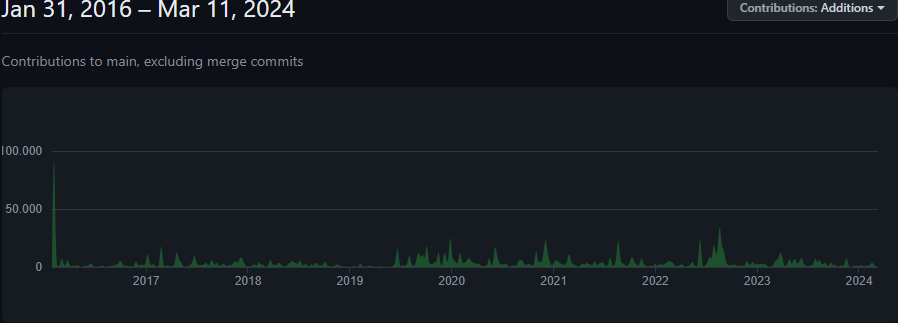
\includegraphics[width=0.75\linewidth]{source/implementation/evaluation/postgresql_ha_solutions/insights/stackgres_citus/contributors_additions_citusdata_citus}
        \caption{Citus - Contributors Additions}
        \label{fig:contributors_additions_citusdata_citus}
    \end{figure}

    Gerade Ende Januar gab es bei Stackgres eine grössere Anzahl Commits, anhand der statistik wird ersichtlich, dass i.d.R. einmal pro Monat grössere Mengen an Commits eingespielt werden.
    Bei Citus gibt es ebenfalls Regelmässig grössere Mengen an Commits, allerdings scheint bei citusdata mehr mit kürzeren Sprints gearbeitet zu werden als bei ongres denn die Commits sind Regelmässiger:
    \begin{figure}[H]
        \centering
        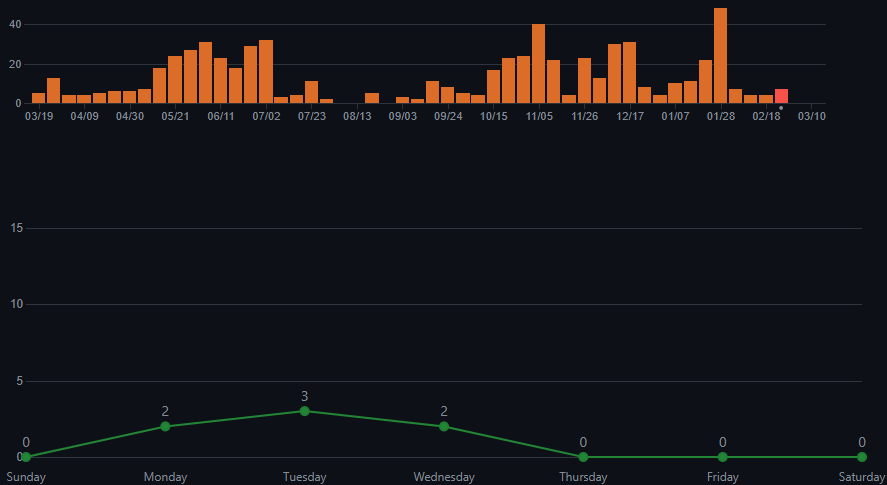
\includegraphics[width=0.75\linewidth]{source/implementation/evaluation/postgresql_ha_solutions/insights/stackgres_citus/commit_activity_ongres_stackgres}
        \caption{Stackgres - Commit Activity}
        \label{fig:commit_activity_ongres_stackgres}
    \end{figure}
    \begin{figure}[H]
        \centering
        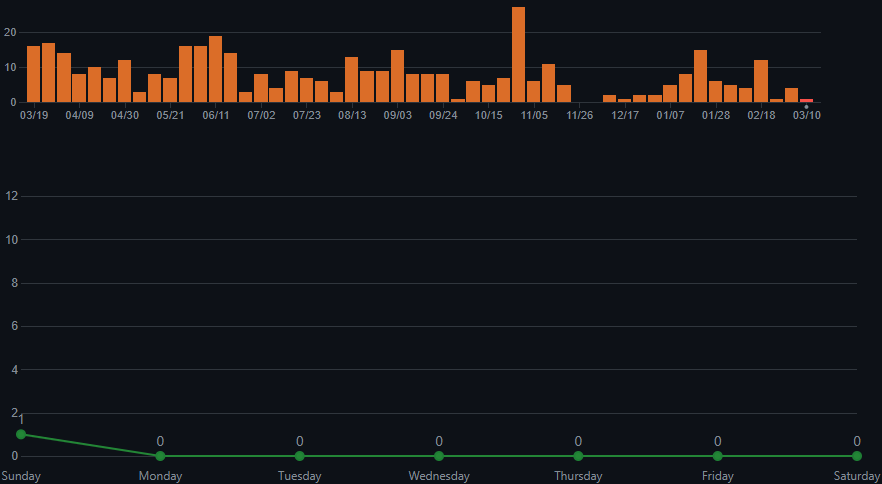
\includegraphics[width=0.75\linewidth]{source/implementation/evaluation/postgresql_ha_solutions/insights/stackgres_citus/commit_activity_citusdata_citus}
        \caption{Citus - Commit Activity}
        \label{fig:commit_activity_citusdata_citus}
    \end{figure}

    In letzter Zeit haben nur ongres, der Entwickler von Stackgres, als auch citusdata, grössere Commits auf das Repository gefahren.
    Andere grössere Entwickler wie EnterpriseDB sind abwesend.
    \begin{figure}[H]
        \centering
        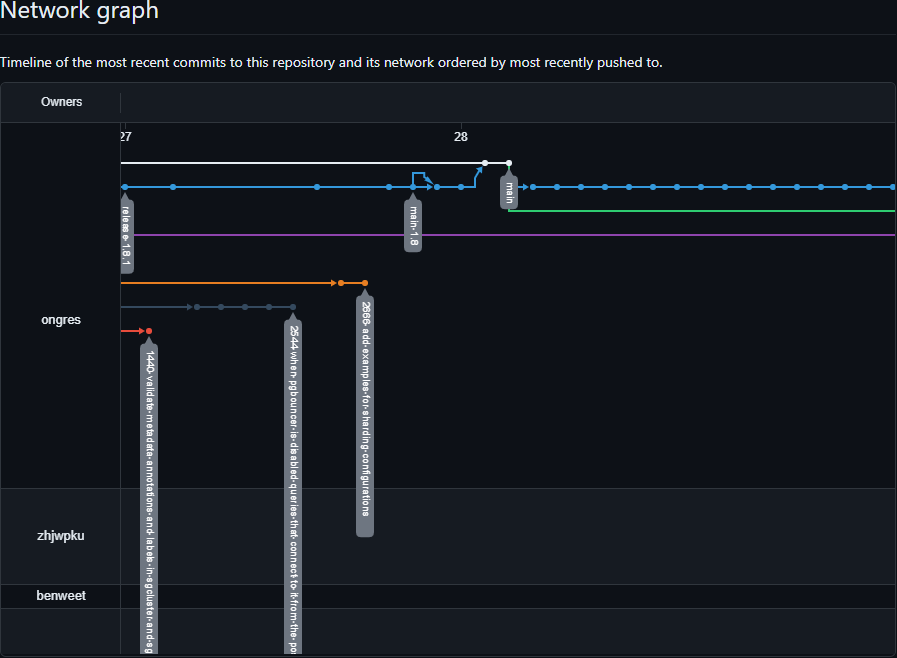
\includegraphics[width=0.75\linewidth]{source/implementation/evaluation/postgresql_ha_solutions/insights/stackgres_citus/network_graph_ongres_stackgres}
        \caption{Stackgres - Network Graph}
        \label{fig:network_graph_ongres_stackgres}
    \end{figure}
    \begin{figure}[H]
        \centering
        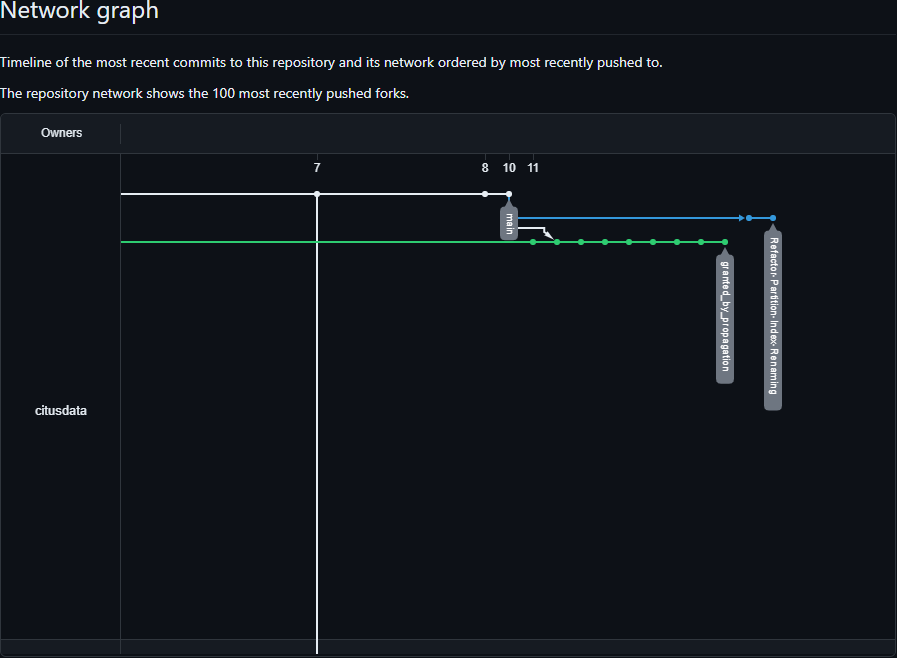
\includegraphics[width=0.75\linewidth]{source/implementation/evaluation/postgresql_ha_solutions/insights/stackgres_citus/network_graph_citusdata_citus}
        \caption{Citus - Network Graph}
        \label{fig:network_graph_citusdata_citus}
    \end{figure}

\end{flushleft}
%! Author = gramic
%! Date = 11.03.24

% Preamble
\begin{flushleft}
    \subsection{Vorauswahl}
    Folgende Lösungen werden nicht evaluiert, sondern bereits zu Beginn ausgeschieden:
    \begin{table}[H]

\resizebox{\columnwidth}{!}{%

\begin{tabular}{rlll}
\toprule
Nr. & Lösung & Status & Begründung \\
\midrule
1 & KSGR-Lösung & Vorausgeschieden & \begin{tabular}[c]{@{}l@{}}Hat nur einen Standy / Replika-Node.\\Failover Funktioniert nur bei kleineren Datenmengen wirklich in einer vernüftigen Zeit.\end{tabular} \\
2 & pgpool-II & Vorausgeschieden & \begin{tabular}[c]{@{}l@{}}pgpool-II hat kein GitHub-Repository und bietet daher keine vergleichswerte mittels Github Insights.\end{tabular} \\
3 & pg\_auto\_failover & Vorausgeschieden & \begin{tabular}[c]{@{}l@{}}pg\_auto\_failover würde zwar Citus-Support bieten,\\allerdings gibt es keine gut dokumentierte Implementation für Kubernetes.\\Erfüllt daher das Kriterium für die Synergien nicht\end{tabular} \\
4 & CloudNativePG & Vorausgeschieden & \begin{tabular}[c]{@{}l@{}}CloudNativePG ist keine vollständige Cloud Native Lösung.\\Mittels Citus könnte sogar eine Distributed SQL Lösung implementiert werden.\\Die Grundarchitektur bleibt aber Monolithisch mit einem Primary und Replikas.\\Und da kein Benefit in Form von Synergien vorhanden sind,\\fällt CloudNativePG raus.\end{tabular} \\
8 & Citus row-based-sharding & Vorausgeschieden & \begin{tabular}[c]{@{}l@{}}Citus row-based-sharding wäre Hocheffizient\\wenn es um Ressourcenverteilung geht und zudem echtes Sharding.\\Allerdings setzt es anpassungen an den Tabellen der Applikationen voraus.\\Das KSGR ist allerdings kein Softwarehaus\\und kann keine Forks durchführen,\\auch weil viele Applikationen zertifiziert sein müssen.\\Scheitert daher an der Machbarkeit\end{tabular} \\
\bottomrule
\end{tabular}
}
\caption{Vorauswahl - Ausgeschieden} \label{predecision_out}
\end{table}


    Entsprechend werden nur noch nachfolgende Lösungen genauer betrachtet:
    \begin{table}[H]

\resizebox{\columnwidth}{!}{%

\begin{tabular}{rlll}
\toprule
Nr. & Lösung & Status & Begründung \\
\midrule
4 & Patroni & Evaluation & \begin{tabular}[c]{@{}l@{}}Patroni kann als Monolithisches System genutzt werden,\\ist aber auch Kern von Stackgres.\\Die API und Skripte können also in beiden Welten verwendet werden\end{tabular} \\
5 & Stackgres mit Citus & Evaluation & \begin{tabular}[c]{@{}l@{}}Bietet eine einfache und kompakte Möglichkeit für ein Distributed SQL System.\\Da Patroni unter der Haube ist,\\kann die API und sonstige Skripte auch auf einem Monolithischen System eingesetzt werden.\end{tabular} \\
6 & Yugabyte-DB & Evaluation & \begin{tabular}[c]{@{}l@{}}Ist eine reine Distributed SQL Lösung und ist Vollständig Cloud Native.\end{tabular} \\
\bottomrule
\end{tabular}
}
\caption{Vorauswahl - Evaluation} \label{predecision_in}
\end{table}

\end{flushleft}
\subsection{Installation verschiedener Lösungen}
%! Author = itgramic
%! Date = 26.01.24

% Preamble
\subsubsection{Monolitische Umgebung}
\subsubsection{Kubernetes}
Um ein minimales, dem Produktiven möglichst nahes Enviroment für die evaluation zu erhalten, wurde folgendes Setting ausgewählt:
\begin{table}[]
\begin{tabular}{ll}
\textbf{Linux Distribution}                & Debian 11              \\
\textbf{Kubernetes Runtime}                & rke2                   \\
\textbf{Container-Enviroment}              & containerd             \\
\textbf{Container Network Interface (CNI)} & cilium                 \\
\textbf{Cloud Native Storage (CNS)}        & local-path-provisioner
\end{tabular}
\caption{Evaluations settings}
\label{tab:evaluation-setting}
\end{table}
%! Author = gramic
%! Date = 15.03.24

% Preamble
\begin{flushleft}
    \subsubsection{rke2 - Evaluationsplattform}
    Die Grundsätzliche Evaluationsplattform für Distributed SQL / Shards sieht folgendermassen aus:
    \begin{figure}[H]
        \centering
        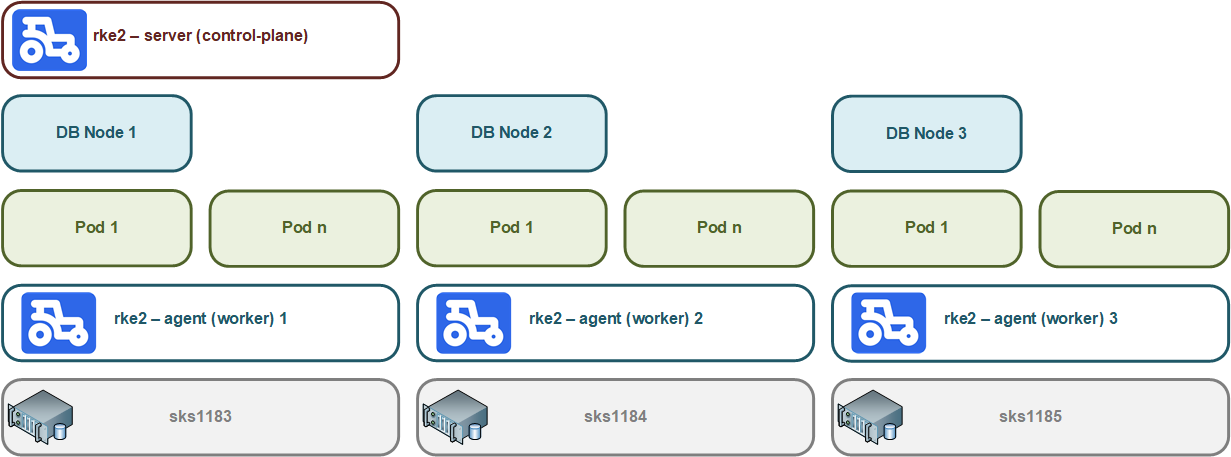
\includegraphics[width=0.8\linewidth]{source/implementation/evaluation/platforms/evaluation_enviroment_rke2}
        \caption{Evaluationssystem - Distributed SQL / Shards}
        \label{fig:evaluation_enviroment_rke2}
    \end{figure}
    
    Die Konfiguration der rke2-Nodes sieht folgendermassen aus:
    \begin{table}[H]


\begin{tabular}{ll}
\toprule
\midrule
\textbf{Kubernetes Runtime} & rke2 \\
\textbf{Container-Enviroment} & containerd \\
\textbf{Container Network Interface (CNI)} & cilium \\
\textbf{loud Native Storage (CNS)} & local-path-provisioner \\
\bottomrule
\end{tabular}
\caption{Evaluationssysstem - Distributed SQL / Sharding} \label{evaluation_distributed_sql}
\end{table}

    
\end{flushleft}
%! Author = gramic
%! Date = 15.03.24

% Preamble
\clearpage
\KOMAoptions{paper=A4,paper=portrait,pagesize}
\recalctypearea
\begin{flushleft}
    \subsubsection{Patroni}
    \paragraph{Architektur}
    Ursprünglich sollte auf jedem Patroni Server (\texttt{sks1232}, \texttt{sks1233} und \texttt{sks1234}) ein \gls{etcd}-Node installiert werden.\\
    Auch sollte auf \texttt{sks1234} der \Gls{HAProxy} installiert werden.\\
    Im Kapitel \hyperref[par:patroni_installation]{Installation} wird erklärt, wieso die Architektur nun folgendermassen aussieht:
    \begin{figure}[H]
        \centering
        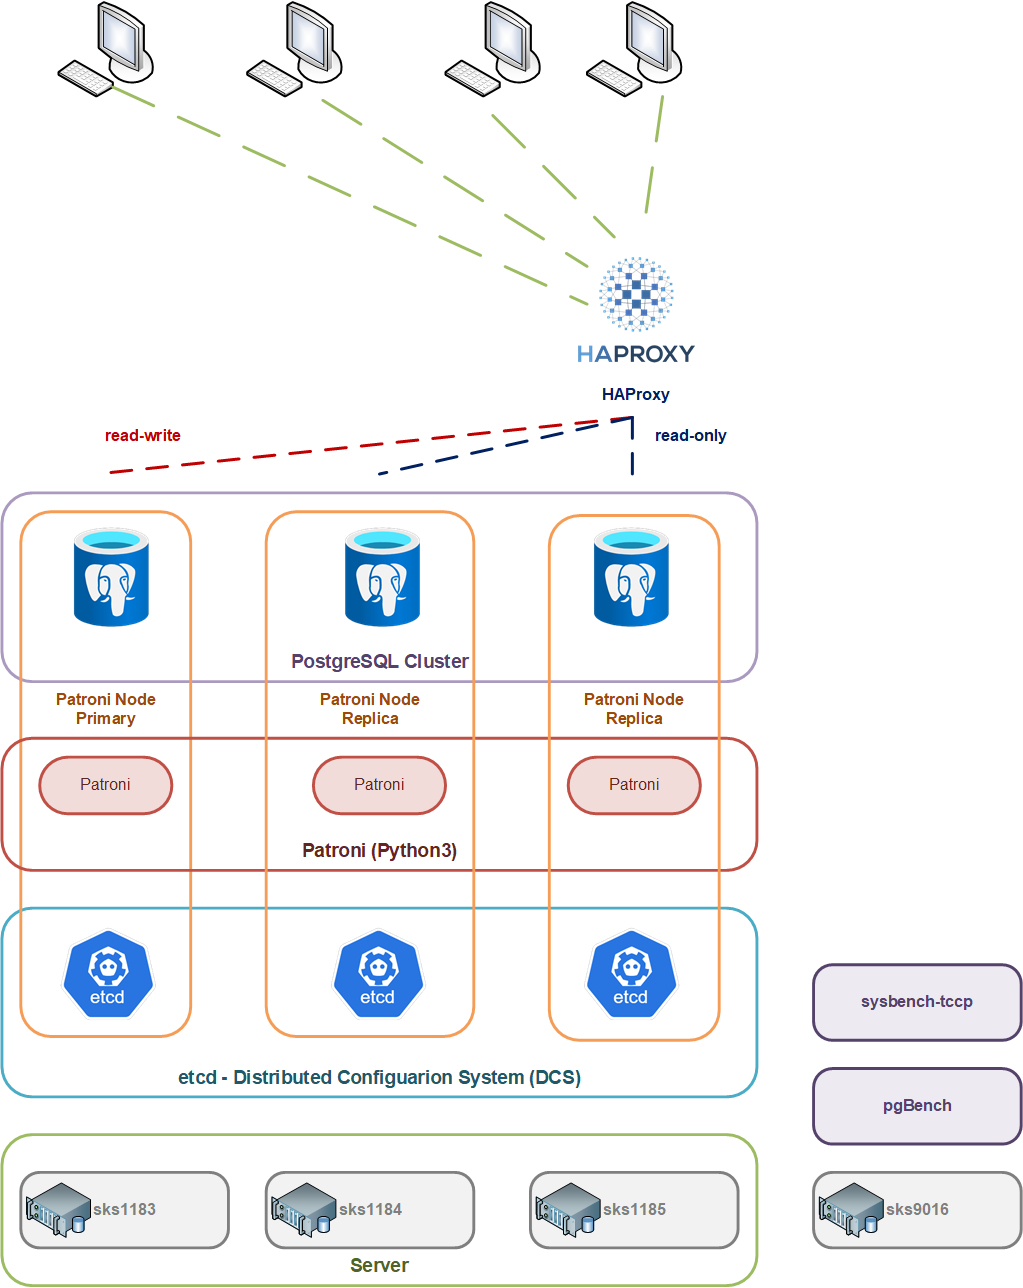
\includegraphics[width=0.8\linewidth]{source/implementation/evaluation/postgresql_ha_solutions/patroni/patroni-evaluation-architecture}
        \caption{Patroni - Evaluationsarchitektur}
        \label{fig:patroni-evaluation-architecture.png}
    \end{figure}
    Neu wird auf \texttt{sks9016} ein \gls{etcd}-Node und der \Gls{HAProxy} installiert.
\end{flushleft}
%\clearpage
%\KOMAoptions{paper=A4,paper=portrait,pagesize}
%\recalctypearea
\clearpage
\begin{flushleft}
    \paragraph{Installation}
    \label{par:patroni_installation}
    Wie schon erwähnt, wurde versucht die \gls{etcd}-Nodes auf die Patroni-Nodes zu installieren.
\end{flushleft}
%\clearpage
%\KOMAoptions{paper=A4,paper=portrait,pagesize}
%\recalctypearea
\begin{flushleft}
    Erst kam es zu einem Fehler, dass keine Verbindung zum \gls{etcd}-Node hergestellt werden konnte:
\lstset{style=gra_codestyle}
\begin{lstlisting}[language=bash, caption=Patroni - etcd API V2 Error,captionpos=b,label={lst:patroni_etcd_api_v2_error},breaklines=true]
ERROR: Failed to get list of machines from http://10.0.20.110:2379/v2: EtcdException('Bad response : 404 page not found\n')
INFO: waiting on etcd
\end{lstlisting}
    Ursache war, dass \gls{etcd} V3 ab Version v3.4 die API V2 nicht mehr per Default aktiv ist.
    Man könnte bis v3.7 die API V2 noch aktivieren:
\lstset{style=gra_codestyle}
\begin{lstlisting}[language=bash, caption=Patroni - etcd API V2 Enable,captionpos=b,label={lst:patroni_etcd_api_v2_enable},breaklines=true]
ETCDCTL_API=2
\end{lstlisting}
    Die nachhaltigere Lösung ist, im Konfiguations-yml-File des Patroni-Nodes Version 3 zu setzen (und dieses Package auch explizit zu installieren):
\lstset{style=gra_codestyle}
\begin{lstlisting}[language=yaml, caption=Patroni - etcd3 Flag,captionpos=b,label={lst:patroni_etcd3_flag},breaklines=true]
...
etcd3:
    host: <ip / hostname>:2379
...
\end{lstlisting}
\end{flushleft}
%\clearpage
%\KOMAoptions{paper=A4,paper=portrait,pagesize}
%\recalctypearea
\begin{flushleft}
    Der Primary-Node konnte in jeden Fall installiert und deployt werden.
    Sobald aber jeweils die Replika-Nodes gestartet wurden, kam es zu einem Fehler.
    Die Ursache war, dass es ja bereits einen Host-Key für den jeweiligen Hostnamen resp.
    die entsprechende IP gab, nämlich den \gls{etcd}-Node.
    So kam es jeweils zu einem Key-Error.
    Nach einigem Versuchen, etwa die Keys neu zu beschreiben, brach ich die Übung ab.
    Der \gls{etcd}-Node wurde nun nur noch auf dem Server \texttt{sks9060} installiert.
    Resultat war, dass der Cluster lauffähig wurde.
%    Daraus nehme ich für die ganze Arbeit folgende Erkenntnis heraus, wenn ein System nicht lauffähig gemacht werden kann:\\
%    \textlarger{\textit{\say{Im Zweifelsfall die Komplexität herausnehmen und das ganze System so weit vereinfachen, bis es funktioniert}}}
\end{flushleft}
%\clearpage
%\KOMAoptions{paper=A4,paper=portrait,pagesize}
%\recalctypearea
\begin{flushleft}
    Passwörter können mit dem Bootstrap mitgegeben werden.
    Dazu muss im \texttt{postgresql}-Segment das Subsegment \texttt{authentication} erstellt werden.
    Der Replikationsuser muss mit einem subsegment \texttt{replication} und der postgres-User mit \texttt{superuser} angegeben werden:
\lstset{style=gra_codestyle}
\begin{lstlisting}[language=yaml, caption=Patroni - Passwörter,captionpos=b,label={lst:patroni_passwords},breaklines=true]
...
postgresql:
    ...
    authentication:
        replication:
            username: replicator
            password: <password>
        superuser:
            username: postgres
            password: <password>
...
\end{lstlisting}
\end{flushleft}
%\clearpage
\KOMAoptions{paper=A4,paper=portrait,pagesize}
\recalctypearea
\begin{flushleft}
    Zuerst lief der Cluster nur asynchron, auch die ersten beiden Benchmarks wurden so ausgeführt.
    Der Cluster lässt sich nämlich nicht synchron Bootstrapen, die Konfiguration muss nachträglich gemacht werden.
    Dazu kann ein JSON mit den geänderten Konfiguration übergeben werden, in dieser Konfiguration musste dabei das yml-File mit der Konfiguration angegeben werden:
\lstset{style=gra_codestyle}
\begin{lstlisting}[language=bash, caption=Patroni - Synchrone Replikation setzen,captionpos=b,label={lst:patroni_set_sync_replication},breaklines=true]
patronictl -c /etc/patroni/config.yml edit-config --apply - --force <<'JSON'
{
 synchronous_mode: "on",
 synchronous_mode_strict: "on",
 synchronous_node_count: 2,
 "postgresql":
   {
   "parameters":{
     "synchronous_commit": "on",
     "synchronous_standby_names": "*"
   }
  }
}
JSON
\end{lstlisting}
\end{flushleft}
%\clearpage
%\KOMAoptions{paper=A4,paper=portrait,pagesize}
%\recalctypearea
\begin{flushleft}
    Die Vergrösserung der Disks hat nur einen begrenzten Impact.
    Lediglich das Verzeichnis \texttt{pg\_wal}, welches die \texttt{WAL}-Files aufnimmt, muss angepasst werden.
    Um die Umstellung ohne Reinstallation durchführen zu können, muss mit symlinks gearbeitet werden.
    Die Daten können via Tablespace auf die grösseren mounts gesetzt werden.
\end{flushleft}
%\clearpage
%\KOMAoptions{paper=A4,paper=portrait,pagesize}
%\recalctypearea
\begin{flushleft}
    Die vollständige Dokumentation der Evaluationsinstallation ist im \hyperref[subsec:evaluation_installation_patroni]{Anhang - Installation Patroni} zu finden.
\end{flushleft}
\subsubsection{Stackgres mit Citus}
\begin{flushleft} 
Stackgres ist eine PostgreSQL Implementation die dafür vorgesehenen ist, in einem Kubernetes Cluster betrieben zu werden.
\end{flushleft} 
\begin{flushleft}
An sich wäre Stackgres nur eine Implementation von Patroni in Kubernetes inkl. Load Balancer.\\
Nun kommt das Citus-Plugin ins spiel, welches aus einer jeden Monolithischen, Klassischen PostgreSQL Installation eine Distributed SQL Umgebung macht.////
Citus wiederum ist in den Microsoft Konzern eingebettet
\end{flushleft}

\begin{flushleft}
    \paragraph{Architektur}
    \begin{flushleft}
        \subparagraph{Citus Coordinator und Workers}
        \begin{figure}[H]
            \centering
            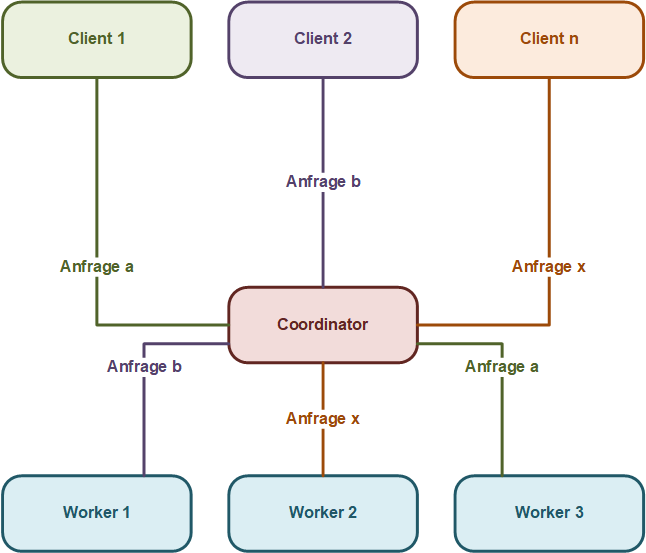
\includegraphics[width=0.75\linewidth]{source/implementation/evaluation/postgresql_ha_solutions/stackgres/citus_coordinator_worker}
            \caption{Citus - Coordinator und Workers}
            \label{fig:citus_coordinator_worker}
        \end{figure}
    \end{flushleft}
    \begin{flushleft}
        \subparagraph{Citus Sharding}
        Citus bietet zwei Sharding-Modelle an.
        \begin{flushleft}
            \textbf{Row-based sharding}
            Beim diesen sharding werden Tabellen anhand einer Distribution Column aufgeteilt. \cite{2Y5FA36C, FDUUL9IM}
        \end{flushleft}
        \begin{flushleft}
            \textbf{Schema-based sharding}
        \end{flushleft}
    \end{flushleft}
\end{flushleft}
\begin{flushleft}
    \paragraph{Maintenance}
    Bei Stackgres gab es im letzten Monat keine wirkliche Bewegung:
    \begin{figure}[H]
        \centering
        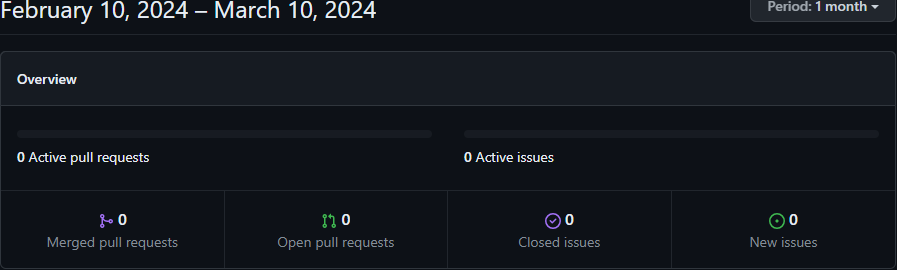
\includegraphics[width=0.75\linewidth]{source/implementation/evaluation/postgresql_ha_solutions/insights/stackgres_citus/pulse_ongres_stackgres}
        \caption{Stackgres - Pulse}
        \label{fig:pulse_ongres_stackgres}
    \end{figure}
    Anders sieht es bei Citus aus, die Firma die mittlerweile zu Microsoft gehört, schliesst Issues rasch und hat eine verhältnissmässig hohe Requstrate:
    \begin{figure}[H]
        \centering
        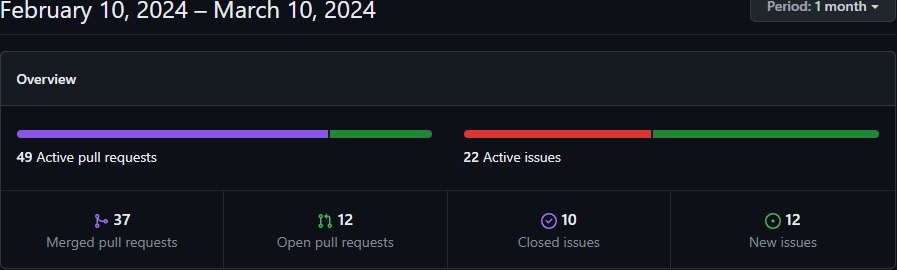
\includegraphics[width=0.75\linewidth]{source/implementation/evaluation/postgresql_ha_solutions/insights/stackgres_citus/pulse_citusdata_citus}
        \caption{Citus - Pulse}
        \label{fig:pulse_citusdata_citus}
    \end{figure}

    Bei Stackgres wird sehr viel Code hinzugefügt oder gelöscht, beim älteren Citus wurden weniger änderungen verzeichnet:
    \begin{figure}[H]
        \centering
        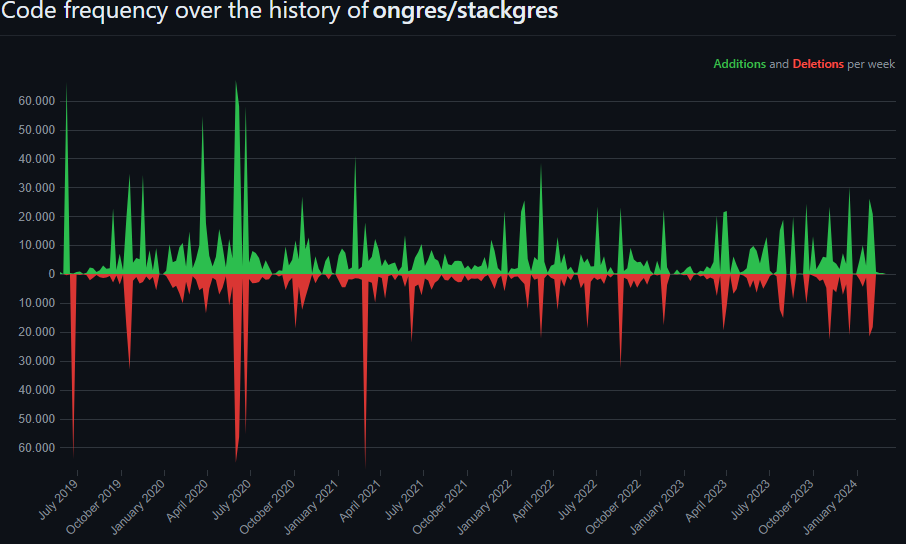
\includegraphics[width=0.75\linewidth]{source/implementation/evaluation/postgresql_ha_solutions/insights/stackgres_citus/code_frequency_ongres_stackgres}
        \caption{Stackgres - Code Frequency}
        \label{fig:code_frequency_ongres_stackgres}
    \end{figure}
    \begin{figure}[H]
        \centering
        \includegraphics[width=0.75\linewidth]{source/implementation/evaluation/postgresql_ha_solutions/insights/stackgres_citus/code_frequency_citusdata_citus}
        \caption{Citus - Code Frequency}
        \label{fig:code_frequency_citusdata_citus}
    \end{figure}

    Citus legt einen hohen Stellenwert auf die Community-Standars, Stackgres selbst schneidet hier nur Mittelmässig ab:
    \begin{figure}[H]
        \centering
        \includegraphics[width=0.75\linewidth]{source/implementation/evaluation/postgresql_ha_solutions/insights/stackgres_citus/stackgres_community_standards}
        \caption{Stackgres - Community Standards}
        \label{fig:stackgres_community_standards}
    \end{figure}
    \begin{figure}[H]
        \centering
        \includegraphics[width=0.75\linewidth]{source/implementation/evaluation/postgresql_ha_solutions/insights/stackgres_citus/citus_community_standards}
        \caption{Citus - Community Standards}
        \label{fig:citus_community_standards}
    \end{figure}

    Die Stackgres Constributors pflegen aktiv Additions ein, löschen Regelmässig und Commiten ebenfalls auf die main-Branch.
    Citus, dessen Repository länger Commited wird, hat weniger bewegung auf die main-Branch.
    \begin{figure}[H]
        \centering
        \includegraphics[width=0.75\linewidth]{source/implementation/evaluation/postgresql_ha_solutions/insights/stackgres_citus/contributors_commits_ongres_stackgres}
        \caption{Stackgres - Contributors Commits}
        \label{fig:contributors_commits_ongres_stackgres}
    \end{figure}
    \begin{figure}[H]
        \centering
        \includegraphics[width=0.75\linewidth]{source/implementation/evaluation/postgresql_ha_solutions/insights/stackgres_citus/contributors_deletations_ongres_stackgres}
        \caption{Stackgres - Contributors Deletations}
        \label{fig:contributors_deletations_ongres_stackgres}
    \end{figure}
    \begin{figure}[H]
        \centering
        \includegraphics[width=0.75\linewidth]{source/implementation/evaluation/postgresql_ha_solutions/insights/stackgres_citus/contributors_addition_ongres_stackgres}
        \caption{Stackgres - Contributors Additions}
        \label{fig:contributors_addition_ongres_stackgres}
    \end{figure}
    \begin{figure}[H]
        \centering
        \includegraphics[width=0.75\linewidth]{source/implementation/evaluation/postgresql_ha_solutions/insights/stackgres_citus/contributors_commits_citusdata_citus}
        \caption{Citus - Contributors Commits}
        \label{fig:contributors_commits_citusdata_citus}
    \end{figure}
    \begin{figure}[H]
        \centering
        \includegraphics[width=0.75\linewidth]{source/implementation/evaluation/postgresql_ha_solutions/insights/stackgres_citus/contributors_deletations_citusdata_citus}
        \caption{Citus - Contributors Deletations}
        \label{fig:contributors_deletations_citusdata_citus}
    \end{figure}
    \begin{figure}[H]
        \centering
        \includegraphics[width=0.75\linewidth]{source/implementation/evaluation/postgresql_ha_solutions/insights/stackgres_citus/contributors_additions_citusdata_citus}
        \caption{Citus - Contributors Additions}
        \label{fig:contributors_additions_citusdata_citus}
    \end{figure}

    Gerade Ende Januar gab es bei Stackgres eine grössere Anzahl Commits, anhand der statistik wird ersichtlich, dass i.d.R. einmal pro Monat grössere Mengen an Commits eingespielt werden.
    Bei Citus gibt es ebenfalls Regelmässig grössere Mengen an Commits, allerdings scheint bei citusdata mehr mit kürzeren Sprints gearbeitet zu werden als bei ongres denn die Commits sind Regelmässiger:
    \begin{figure}[H]
        \centering
        \includegraphics[width=0.75\linewidth]{source/implementation/evaluation/postgresql_ha_solutions/insights/stackgres_citus/commit_activity_ongres_stackgres}
        \caption{Stackgres - Commit Activity}
        \label{fig:commit_activity_ongres_stackgres}
    \end{figure}
    \begin{figure}[H]
        \centering
        \includegraphics[width=0.75\linewidth]{source/implementation/evaluation/postgresql_ha_solutions/insights/stackgres_citus/commit_activity_citusdata_citus}
        \caption{Citus - Commit Activity}
        \label{fig:commit_activity_citusdata_citus}
    \end{figure}

    In letzter Zeit haben nur ongres, der Entwickler von Stackgres, als auch citusdata, grössere Commits auf das Repository gefahren.
    Andere grössere Entwickler wie EnterpriseDB sind abwesend.
    \begin{figure}[H]
        \centering
        \includegraphics[width=0.75\linewidth]{source/implementation/evaluation/postgresql_ha_solutions/insights/stackgres_citus/network_graph_ongres_stackgres}
        \caption{Stackgres - Network Graph}
        \label{fig:network_graph_ongres_stackgres}
    \end{figure}
    \begin{figure}[H]
        \centering
        \includegraphics[width=0.75\linewidth]{source/implementation/evaluation/postgresql_ha_solutions/insights/stackgres_citus/network_graph_citusdata_citus}
        \caption{Citus - Network Graph}
        \label{fig:network_graph_citusdata_citus}
    \end{figure}

\end{flushleft}
%! Author = gramic
%! Date = 15.03.24

% Preamble
\begin{flushleft}
    \subsubsection{yugabyteDB}
    \paragraph{Installation}
    Wähend der Installation des YugabyteDB Evaluations-Enviroment wurde festgestellt, das man zwei Varianten Installieren kann.
    YugabyteDB (Repository yugabyte) und YugabyteDB Anywhere (Repository yugawre):
    \begin{figure}[H]
        \centering
        \includegraphics[width=1\linewidth]{source/implementation/evaluation/platforms/yugabytedb_pod_installation_subscription_interrup}
        \caption{yugabyteDB - Susbsription yugawre}
        \label{fig:yugabytedb_pod_installation_subscription_interrup}
    \end{figure}
\end{flushleft}
\begin{flushleft}
    Es stellte sich auch heraus, dass wenn man YugabyteDB 4 Cores pro Node zur Verfügung geben will (je zwei für den \texttt{master} und \texttt{tserver}),\\
    der Server mehr als 4 Cores haben muss.\\
    Andernfalls wird Kubernetes einen der beiden Pods nicht deployen, weil zuwenig Cores zur verfügung stehen.
\end{flushleft}
\begin{flushleft}
    Bei der konstelation \gls{rke2}, \Gls{Cilium} und \Gls{MetalLB}, muss nebst dem \texttt{IPAddressPool} auch ein \texttt{L2Advertisement} für den Pool gesetzt werden.\\
    Ansonsten kann die im YugabyteDB values.yaml gesetzte IP für den \texttt{tserver} von aussen nicht angesprochen werden:
    \lstset{style=gra_codestyle}
    \begin{lstlisting}[language=yaml, caption=metallb - Konfig YAML - Detail L2Advertisement,captionpos=b,label={lst:metallb-l2advertisement-setting},breaklines=true]
---
apiVersion: metallb.io/v1beta1
kind: L2Advertisement
metadata:
  name: l2adv
  namespace: metallb-system
spec:
  ipAddressPools:
  - distributed-sql
    \end{lstlisting}
    Dieses Problem ist schwer zu greifen und hat zwei Tage in Anspruch genommen, es zu Lösen.
    Die Vorschläge zum Lösen des Problems reichten von deakivieren von \texttt{kube-proxy} bis hin zu einer Migration zum \Gls{Cilium}-Loadb-Balancers.\\
    Mit diesem funktionierte dann nicht einmal mehr die Installation von yugabyteDB.\\
    Lösung brachte nur ein \texttt{GitHub}-Eintrag\cite{D4IZIEFN}, wo oben genannter Ansatz empfohlen wurde.
\end{flushleft}
\begin{flushleft}
    \paragraph{Konfiguration}
    Damit nicht der YugabyteDB Anywhere-Service installiert wird, muss das entsprechende Image gesetzt werden:
    \lstset{style=gra_codestyle}
    \begin{lstlisting}[language=yaml, caption=yugabyteDB - Helm Chart Manifest - Detail Image,captionpos=b,label={lst:yugabytedb-image-setting},breaklines=true]
...
Image:
  repository: "yugabytedb/yugabyte"
  tag: 2.20.2.1-b3
  pullPolicy: IfNotPresent
  pullSecretName: ""
...
    \end{lstlisting}

    Die StorageClass muss im \texttt{values.yaml} gesetzt werden, einmal für den \texttt{master} und einmal für den \texttt{tserver}
    \lstset{style=gra_codestyle}
    \begin{lstlisting}[language=yaml, caption=yugabyteDB - Helm Chart Manifest - Detail StorageClass,captionpos=b,label={lst:yugabytedb-storageclass-setting},breaklines=true]
...
storage:
  ephemeral: false  # will not allocate PVs when true
  master:
    count: 1
    size: 3Gi
    storageClass: "yb-storage"
  tserver:
    count: 1
    size: 3Gi
    storageClass: "yb-storage"
...
    \end{lstlisting}

    Dem node werden je 4 Cores zur verfügung gestellt.
    Zei für den \texttt{master} und zwei für den \texttt{tserver}.
    Beide erhalten 4GiB Memory:
    \lstset{style=gra_codestyle}
    \begin{lstlisting}[language=yaml, caption=yugabyteDB - Helm Chart Manifest - Detail Resources,captionpos=b,label={lst:yugabytedb-resources-setting},breaklines=true]
...
resource:
  master:
    requests:
      cpu: "1"
      memory: 2Gi
    limits:
      cpu: "1"
      ## Ensure the 'memory' value is strictly in 'Gi' or 'G' format. Deviating from these formats
      ## may result in setting an incorrect value for the 'memory_limit_hard_bytes' flag.
      ## Avoid using floating numbers for the numeric part of 'memory'. Doing so may lead to
      ## the 'memory_limit_hard_bytes' being set to 0, as the function expects integer values.
      memory: 2Gi
  tserver:
    requests:
      cpu: "1"
      memory: 4Gi
    limits:
      cpu: "1"
      ## Ensure the 'memory' value is strictly in 'Gi' or 'G' format. Deviating from these formats
      ## may result in setting an incorrect value for the 'memory_limit_hard_bytes' flag.
      ## Avoid using floating numbers for the numeric part of 'memory'. Doing so may lead to
      ## the 'memory_limit_hard_bytes' being set to 0, as the function expects integer values.
      memory: 4Gi
...
    \end{lstlisting}

    Die Shards, oder Tablets wie sie Yugabyte nennt, sollen auf allen drei Nodes repliziert werden:
    \lstset{style=gra_codestyle}
    \begin{lstlisting}[language=yaml, caption=yugabyteDB - Helm Chart Manifest - Detail Replika,captionpos=b,label={lst:yugabytedb-replica-setting},breaklines=true]
...
replicas:
  master: 3
  tserver: 3
  ## Used to set replication factor when isMultiAz is set to true
  totalMasters: 3
...
    \end{lstlisting}

    Wichtig ist auch, dass der \texttt{YSQL}-Dienst aktiv ist, damit PostgreSQL Abfragen abgesetzt werden können.\\
    Deshalb muss der Dienst aktiv sein und darf nicht deaktiviert werden:
    \lstset{style=gra_codestyle}
    \begin{lstlisting}[language=yaml, caption=yugabyteDB - Helm Chart Manifest - Detail Disable YSQL,captionpos=b,label={lst:yugabytedb-disableYsql-setting},breaklines=true]
...
# Disable the YSQL
disableYsql: false
...
    \end{lstlisting}

    Nun muss die Domain und die Service-Endpoints konfiguriert werden.\\
    Der Domainname bleibt vorerst \texttt{cluster.local} wie Default hinterlegt.\\
    Die Servicenamen und Ports werden nicht angetastet, wichtig ist die LoadBalancer-IP.\\
    Sie ist entsprechend der gewählten VirtualIP mit \texttt{10.0.20.106} zu setzen.

    \lstset{style=gra_codestyle}
    \begin{lstlisting}[language=yaml, caption=yugabyteDB - Helm Chart Manifest - Detail Domainname und Service-Endpoints,captionpos=b,label={lst:yugabytedb-domainname-serviceendpoints-setting},breaklines=true]
...
domainName: "cluster.local"

serviceEndpoints:
  - name: "yb-master-ui"
    type: LoadBalancer
    annotations: {}
    clusterIP: ""
    ## Sets the Service's externalTrafficPolicy
    externalTrafficPolicy: ""
    app: "yb-master"
    loadBalancerIP: ""
    ports:
      http-ui: "7000"

  - name: "yb-tserver-service"
    type: LoadBalancer
    annotations:
      metallb.universe.tf/loadBalancerIPs: 10.0.20.106
    clusterIP: ""
    ## Sets the Service's externalTrafficPolicy
    externalTrafficPolicy: ""
    app: "yb-tserver"
    loadBalancerIP: ""
    ports:
      tcp-yql-port: "9042"
      tcp-yedis-port: "6379"
      tcp-ysql-port: "5433"
...
    \end{lstlisting}
\end{flushleft}
\begin{flushleft}
    Beim Testen mit der höchsten Anzahl an Datensätzen zeigte sich, dass der \gls{local-path-provisioner} nicht sauber konfiguriert waren.\\
    Damit auf jedem Node die Persistence Volume Claims ausgeführt werden, müssen sie deklariert werden und in den StorageClass-Manifesten auch hinterlegt werden.\\
    Genauer muss in der \texttt{nodePathMap} folgende konfiguration vorgenommen werden:
\lstset{style=gra_codestyle}
\begin{lstlisting}[language=yaml, caption=local-path-provisioner nodePathMap,captionpos=b,label={lst:local-path-provisioner_nodePathMap},breaklines=true]
...
                "nodePathMap":[
                {
                        "node":"DEFAULT_PATH_FOR_NON_LISTED_NODES",
                        "paths":["<Lokaler Pfad>"]
                },
                {
                        "node":"<Nodename>",
                        "paths":["<Lokaler Pfad>"]
                },
...
\end{lstlisting}
    Hier ein Beispiel wie es mit den grossen Volumes aussieht:
\lstset{style=gra_codestyle}
\begin{lstlisting}[language=yaml, caption=local-path-provisioner nodePathMap Beispiel,captionpos=b,label={lst:local-path-provisioner_nodePathMap-exampl},breaklines=true]
...
                "nodePathMap":[
                {
                        "node":"DEFAULT_PATH_FOR_NON_LISTED_NODES",
                        "paths":["/srv/data/local-path-provisioner"]
                },
                {
                        "node":"sks1183",
                        "paths":["/srv/data/local-path-provisioner"]
                },
                {
                        "node":"sks1184",
                        "paths":["/srv/data/local-path-provisioner"]
                },
                {
                        "node":"sks1185",
                        "paths":["/srv/data/local-path-provisioner"]
                }
                ]
...
\end{lstlisting}
    Wird dies nicht gemacht, so wird auf den Default-Path geschrieben.\\
    Das ist zufällig und hat dann zur Folge, dass alle Volumes auf einem Node präsentiert werden.\\
    Was sehr schnell logischerweise dazu führt, dass zuwenig Diskspace vorhanden ist.\\
    Bei YugabyteDB kommt noch dazu, dass es zu Konflikten beim Schreiben von Blocks kommt.
\end{flushleft}
\begin{flushleft}
    Damit die Persistence Volumes sauber präsentiert werden, muss in der StorageClass die \texttt{nodeAffinity} gesetzt werden.\\
    Hier als Beispiel mit den Nodes \texttt{sks1183}, \texttt{sks1184} und \texttt{sks1185}:
\lstset{style=gra_codestyle}
\begin{lstlisting}[language=yaml, caption=yugabyteDB - StorageClass nodeAffinity,captionpos=b,label={lst:yugabytedb-storageclass_example},breaklines=true]
  nodeAffinity:
    required:
      nodeSelectorTerms:
      - matchExpressions:
        - key: kubernetes.io/hostname
          operator: In
          values:
          - sks1183
          - sks1184
          - sks1185
\end{lstlisting}
    \begin{warning}
        \textbf{hostPath}\\
        Der \texttt{hostPath} bei der StorageClass muss der gleiche sein, wie der Pfad im Node des nodePathMap von \gls{local-path-provisioner}.
        Auch sollten die Pfade auf allen Nodes gleich sein.
    \end{warning}
\end{flushleft}
\begin{flushleft}
    Die Problematik mit dem \texttt{nodePathMap} und der \texttt{nodeAffinity} auf der StorageClass hat auch rund zwei Arbeitstage in Anspruch genommen.
\end{flushleft}
%! Author = itgramic
%! Date = 29.12.23

% Preamble
\begin{flushleft}
    \subsection{Entscheid}
    Anhand der Kosten-Nutzen-Analyse, steht die Entscheidung fest.\\
    Patroni wird mit der Variante \texttt{postgresql\_cluster} als Testsystem aufgebaut.
\end{flushleft}
\begin{flushleft}
    Die Umsetzung der Cloud Native Lösung, in diesem Fall YugabyteDB, muss verschoben werden.\\
    Dem \Gls{Kubernetes} Testsystem des KSGR fehlt zum einen noch eine notwendige interne Komponente zur Freigabe,\\
    zum anderen Fehlen für den sauberen Betrieb die Externen Systeme wie der \Gls{PKI} oder dass \Gls{SIEM} (welches aber in den nächsten Wochen eingeführt wird).
\end{flushleft}
\subsection{Gegenüberstellung der Lösungen}
%! Author = itgramic
%! Date = 29.12.23

% Preamble
\begin{flushleft}
    \begin{figure}[H]
        \centering
        \includegraphics[width=1\linewidth]{source/cost_benefit_diagram/cost_benefit_diagram}
        \caption{Kosten-Nutzen-Analyse}
        \label{fig:cost_benefit_diagram}
    \end{figure}
\end{flushleft}
\subsection{Entscheid}